\documentclass[uplatex,dvipdfmx,a4paper,11pt]{jsreport}

\usepackage{docmute}


% 数式
\usepackage{amsmath,amsthm,amssymb}
\usepackage{bm}
% 画像
\usepackage{graphicx}

\usepackage{multirow}
\usepackage{wrapfig}
\usepackage{ascmac}
\usepackage{xcolor}


\usepackage{makeidx}
\makeindex

\graphicspath{{../../_Figures//}{../../_Figures/Rheology/}}

\usepackage{qrcode}
\setlength\lineskiplimit{0pt}
\setlength\normallineskiplimit{0pt}

\usepackage{qexam}

\usepackage{titlesec}
\titleformat*{\section}{\Large\bfseries}
\titleformat*{\subsection}{\large\bfseries}
\titleformat*{\subsubsection}{\normalsize\bfseries}
\titleformat*{\paragraph}{\normalsize\bfseries}

% ページ設定
% \pagestyle{empty}
% 高さの設定
\setlength{\textheight}{\paperheight}   % ひとまず紙面を本文領域に
\setlength{\topmargin}{-5.4truemm}      % 上の余白を20mm(=1inch-5.4mm)に
\addtolength{\topmargin}{-\headheight}  % 
\addtolength{\topmargin}{-\headsep}     % ヘッダの分だけ本文領域を移動させる
\addtolength{\textheight}{-40truemm}    % 下の余白も20mmに%% 幅の設定
\setlength{\textwidth}{\paperwidth}     % ひとまず紙面を本文領域に
\setlength{\oddsidemargin}{-5.4truemm}  % 左の余白を20mm(=1inch-5.4mm)に
\setlength{\evensidemargin}{-5.4truemm} % 
\addtolength{\textwidth}{-40truemm}     % 右の余白も20mmに
% 図と本文との間
%\abovecaptionskip=-5pt
%\belowcaptionskip=-5pt
%
% 全体の行間調整
% \renewcommand{\baselinestretch}{1.0} 
% 図と表
%\renewcommand{\figurename}{Fig.}
%\renewcommand{\tablename}{Tab.}
%

% \makeatletter 
% \def\section{\@startsection {section}{1}{\z@}{1.5 ex plus 2ex minus -.2ex}{0.5 ex plus .2ex}{\large\bf}}
% \def\subsection{\@startsection{subsection}{2}{\z@}{0.2\Cvs \@plus.5\Cdp \@minus.2\Cdp}{0.1\Cvs \@plus.3\Cdp}{\reset@font\normalsize\bfseries}}
% \makeatother 

\usepackage[dvipdfmx,%
 bookmarks=true,%
 bookmarksnumbered=true,%
 colorlinks=false,%
 setpagesize=false,%
 pdftitle={数式に頼らない直感的理解による材料設計のためのレオロジー⼊⾨},%
 pdfauthor={佐々木裕},%
 pdfsubject={},%
 pdfkeywords={レオロジー; 材料設計; }]{hyperref}
\usepackage{pxjahyper}

\usepackage{plext}

\usepackage{niceframe} 
\usepackage{framed}
\newenvironment{longartdeco}{%
  \def\FrameCommand{\fboxsep=\FrameSep \artdecoframe}%
  \MakeFramed {\FrameRestore}}%
 {\endMakeFramed}
 
\usepackage{siunitx}

\newcommand{\rmd}{\mathrm{d}}

\begin{document}

\setcounter{chapter}{6}
\chapter{複雑な事象について}

\section*{この章の内容}

この章では、これまでに行ってきた簡略化したモデルでの議論をベースとして、少しだけ複雑な事象について議論を進めていきましょう。

ここでは、実事象に少しだけ近づくために、流れるということをもう少し詳しく理解することから始めます。
粒子の振る舞いをベースとしたミクロなモデルから、流体の層を切り分けた中間的な大きさの
メゾスケールに注目したモデルへとつなげることで、単純な挙動であるニュートン流動を記述してみます。

その理解に基づいて、非ニュートン流体という、実事象でよく見受けられる複雑な事象を少しだけ理解できるようにつなげていきます。

ここでのお話を具体的に列記すると、以下のような事項となります。
\begin{boxnote}
    \begin{itemize}
		\item 流れるということについて、もう少し
		\begin{itemize}
			\item ニュートン流体を見直しましょう
			\item 流動を表すモデル
			\item 局所的な応力と粘度
		\end{itemize} 
		\item 非ニュートン流体
		\begin{itemize}
			\item 身近な液体とその分類
			\item 非ニュートン流体とは
			\item 非ニュートン性の発現について
		\end{itemize} 
		\item 非ニュートン性と実事象
		\begin{itemize}
			\item 簡単な分類
			\item シア・シニングについて
			\item シア・シックニングについて
		\end{itemize}
	\end{itemize}
\end{boxnote}

\section{流れるということについて、もう少し}

この節では、流れるということについて、もう一度振り返ってみます。
まず、流動現象のモデルとして説明したニュートンの流体モデルについて、中間的なスケールに着目して成り立ちを考えます。

\subsection{ニュートン流体を見直しましょう}

まず、流動を記述するための基本的なモデルであるニュートン保法則についての振り返りから始めていきましょう。

ニュートンの法則とは、以下に示したようなものでした。
\begin{itemize}
	\item せん断応力はせん断速度に比例。
	\item 比例定数の粘度は、せん断速度によらずに一定。
\end{itemize}

これを、数式で書けば、単純な一次方程式の形となるわけです。
\begin{align}
	\text{せん断応力} &= \text{粘度} \times \text{せん断速度} \notag \\
	\tau = \eta \dot{\gamma}
	\label{eq:newton}
\end{align}

具体的な測定においては、図 \ref{fig:newton} に示したような二重円筒のような測定装置で流動特性を評価した場合に、
右に示したように、「せん断速度」の変化に対して、せん断応力は比例し、その比例定数である粘度は一定というグラフになるわけです。
\begin{figure}[htb]
	\begin{center}
		\begin{minipage}{0.45\textwidth}
			\begin{center}
				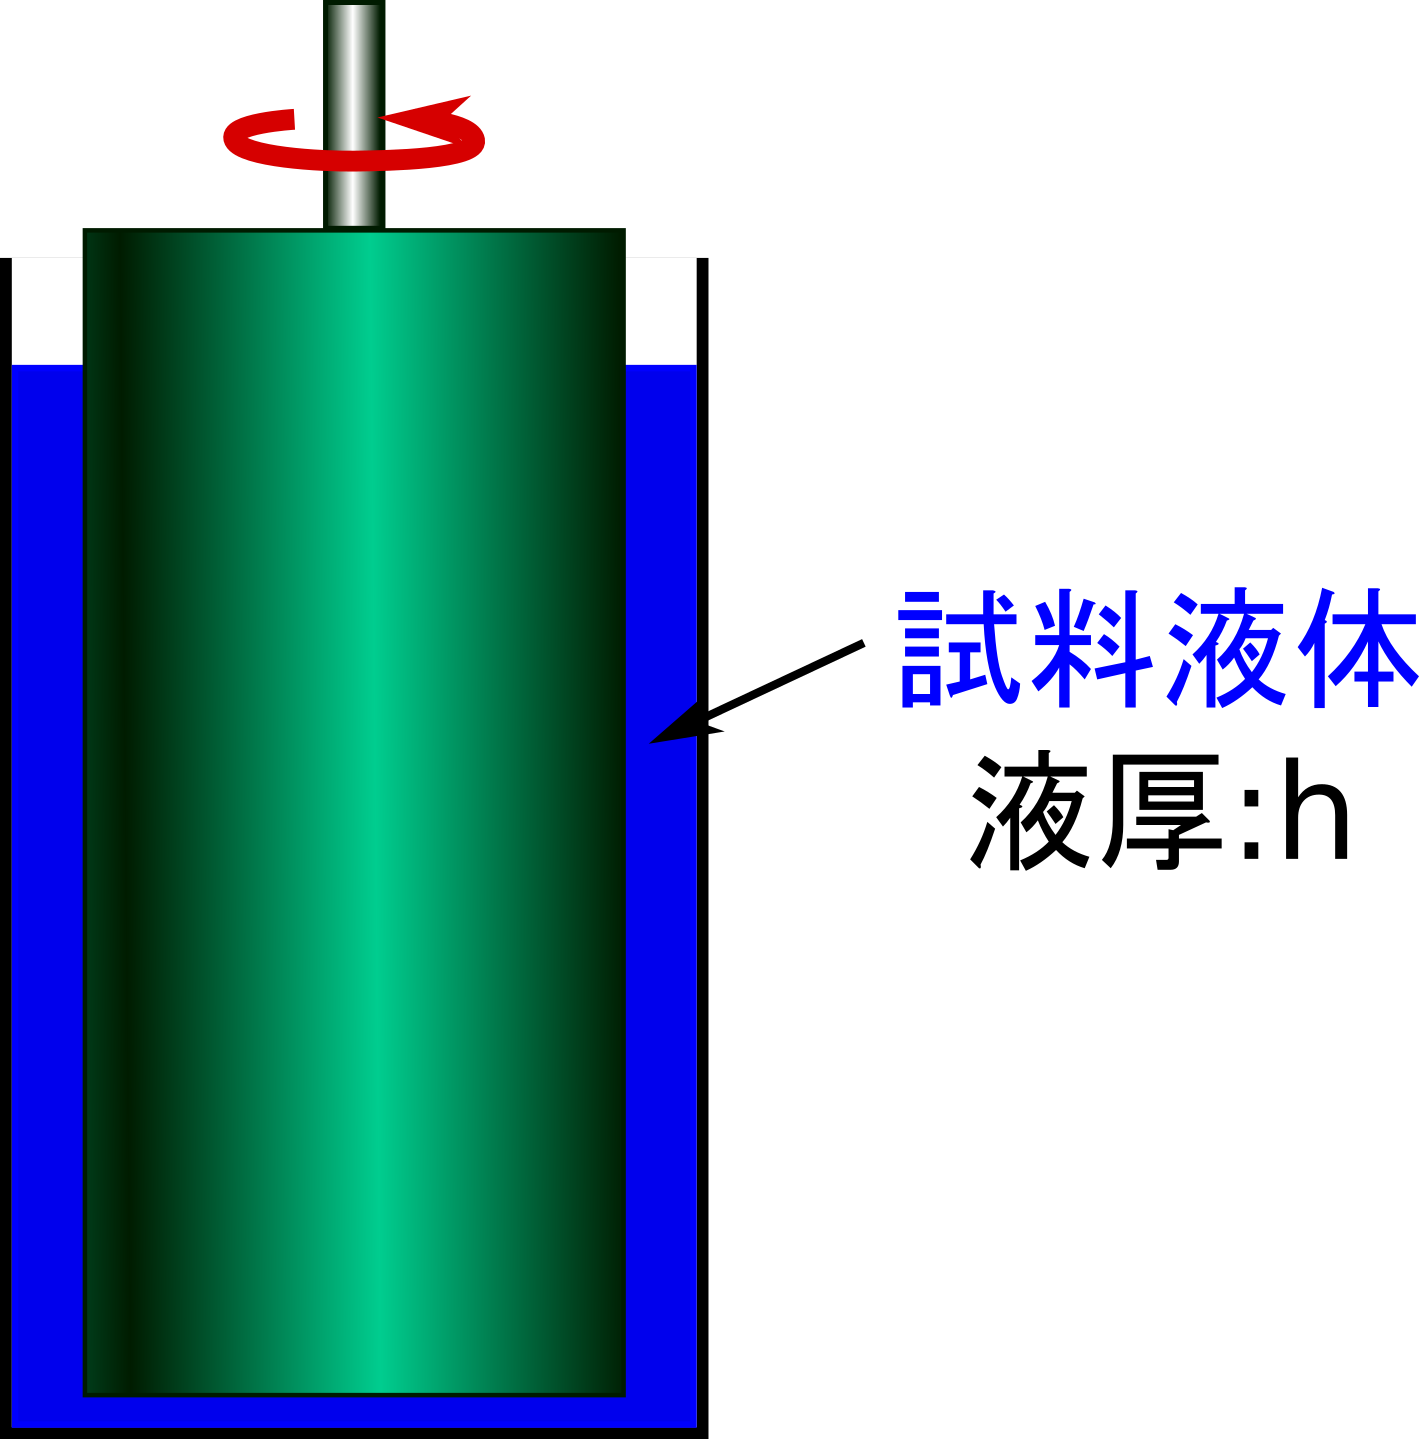
\includegraphics[width=.7\textwidth]{nijyu_entou.png}
				\end{center}
		\end{minipage}
		\begin{minipage}{0.45\textwidth}
			\begin{center}
			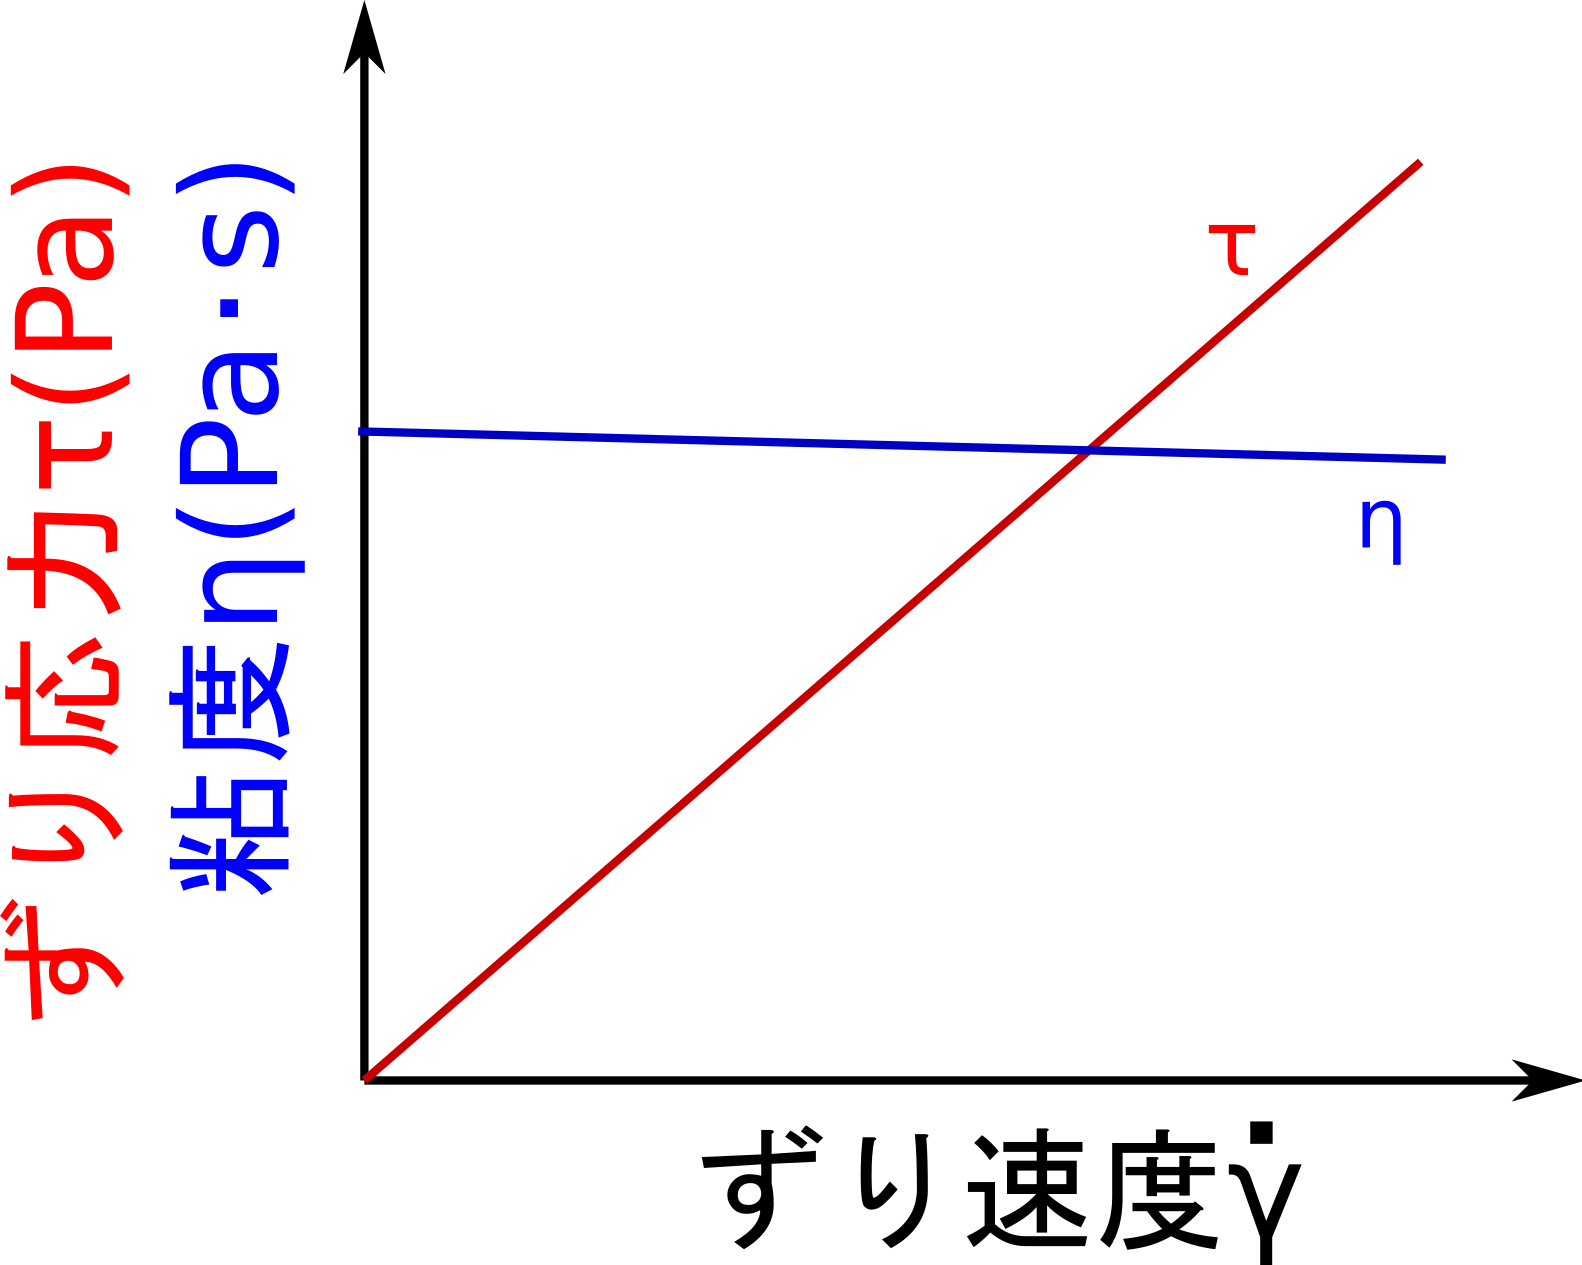
\includegraphics[width=\textwidth]{newtonian.png}
			\end{center}
		\end{minipage}
		\caption{ニュートンの法則}
		\label{fig:newton}
	\end{center}
\end{figure}

\subsection{流動を表すモデル}

液体の流動を表すモデルとして、よく書かれているものは図 \ref{fig:ryudo_model} に示した、水面に板を浮かべた状態を想定したものとなります。
水深方向に n+1 層に分割して、水面の板との境目を 0 とし、水底との境目を n とします。

このとき、注意すべきポイントは、「固体と接している液体は、その相対的な移動速度が同じ」と考えることです。
したがって、「移動する板と接している層 0 は板と同じ速度 $v$ で流れ」、「地面に接している層 $n$ は流れない」ということになります。

そのようなモデルにおいて液体の内部で、それぞれの層ごとに水深に応じて流れる速度、すなわち、仮想的な層の移動速度を考えます。
そして、その層ごとの移動速度がどのように変化するかについて、水深との関係から記述したものが速度勾配というものになります。
最も単純な状態が、その速度分布の勾配が一定の状態となります。

なお、速度勾配は、それぞれの層の速度 $v$ の水深 $y$ への依存性を見たものですから、微分の形で以下のように書くことができます。
\begin{align}
	\dfrac{\mathrm{d} v}{\mathrm{d} y}
	\label{eq:sokudokobai}
\end{align}

また、せん断変形を記述する無次元量であるせん断ひずみ $\gamma$ の時間変化はせん断速度とも呼ばれますが、
これは、以下のようにせん断ひずみを時間で微分したものです。
\begin{align}
	\dfrac{\mathrm{d} \gamma}{\mathrm{d} t} =\dot{\gamma} [s^{-1}]
\end{align}

じつは、この二式は同一のものであり、式 \eqref{eq:sokudokobai} は、以下のように微分の順番を変えることで同一になります。
\begin{align}
	\dfrac{\mathrm{d} v}{\mathrm{d} y} 
	= \dfrac{\mathrm{d} l}{\mathrm{d} t} \dfrac{\mathrm{d} }{\mathrm{d} y}
	= \dfrac{\mathrm{d} l}{\mathrm{d} y} \dfrac{\mathrm{d} }{\mathrm{d} t}
	= \dfrac{\mathrm{d} \gamma}{\mathrm{d} t} =\dot{\gamma} [s^{-1}]
\end{align}


\begin{figure}[htb]
	\begin{center}
		\begin{minipage}{0.45\textwidth}
			\begin{itembox}[l]{水面に板を浮かべたモデル}
				\begin{itemize}
					\item 水深方向に n+1 層に分割
						\begin{itemize}
							\item 水面の板との境目を0
							\item 水底との境目を n 
						\end{itemize}
						\item 液体の内部では、
						\begin{itemize}
							\item 水深に応じて流れる速度の分布
							\item 最も単純な状態:\\速度勾配が一定
						\end{itemize}
				\end{itemize}
			\end{itembox}
		\end{minipage}
		\begin{minipage}{0.45\textwidth}
			\begin{center}
			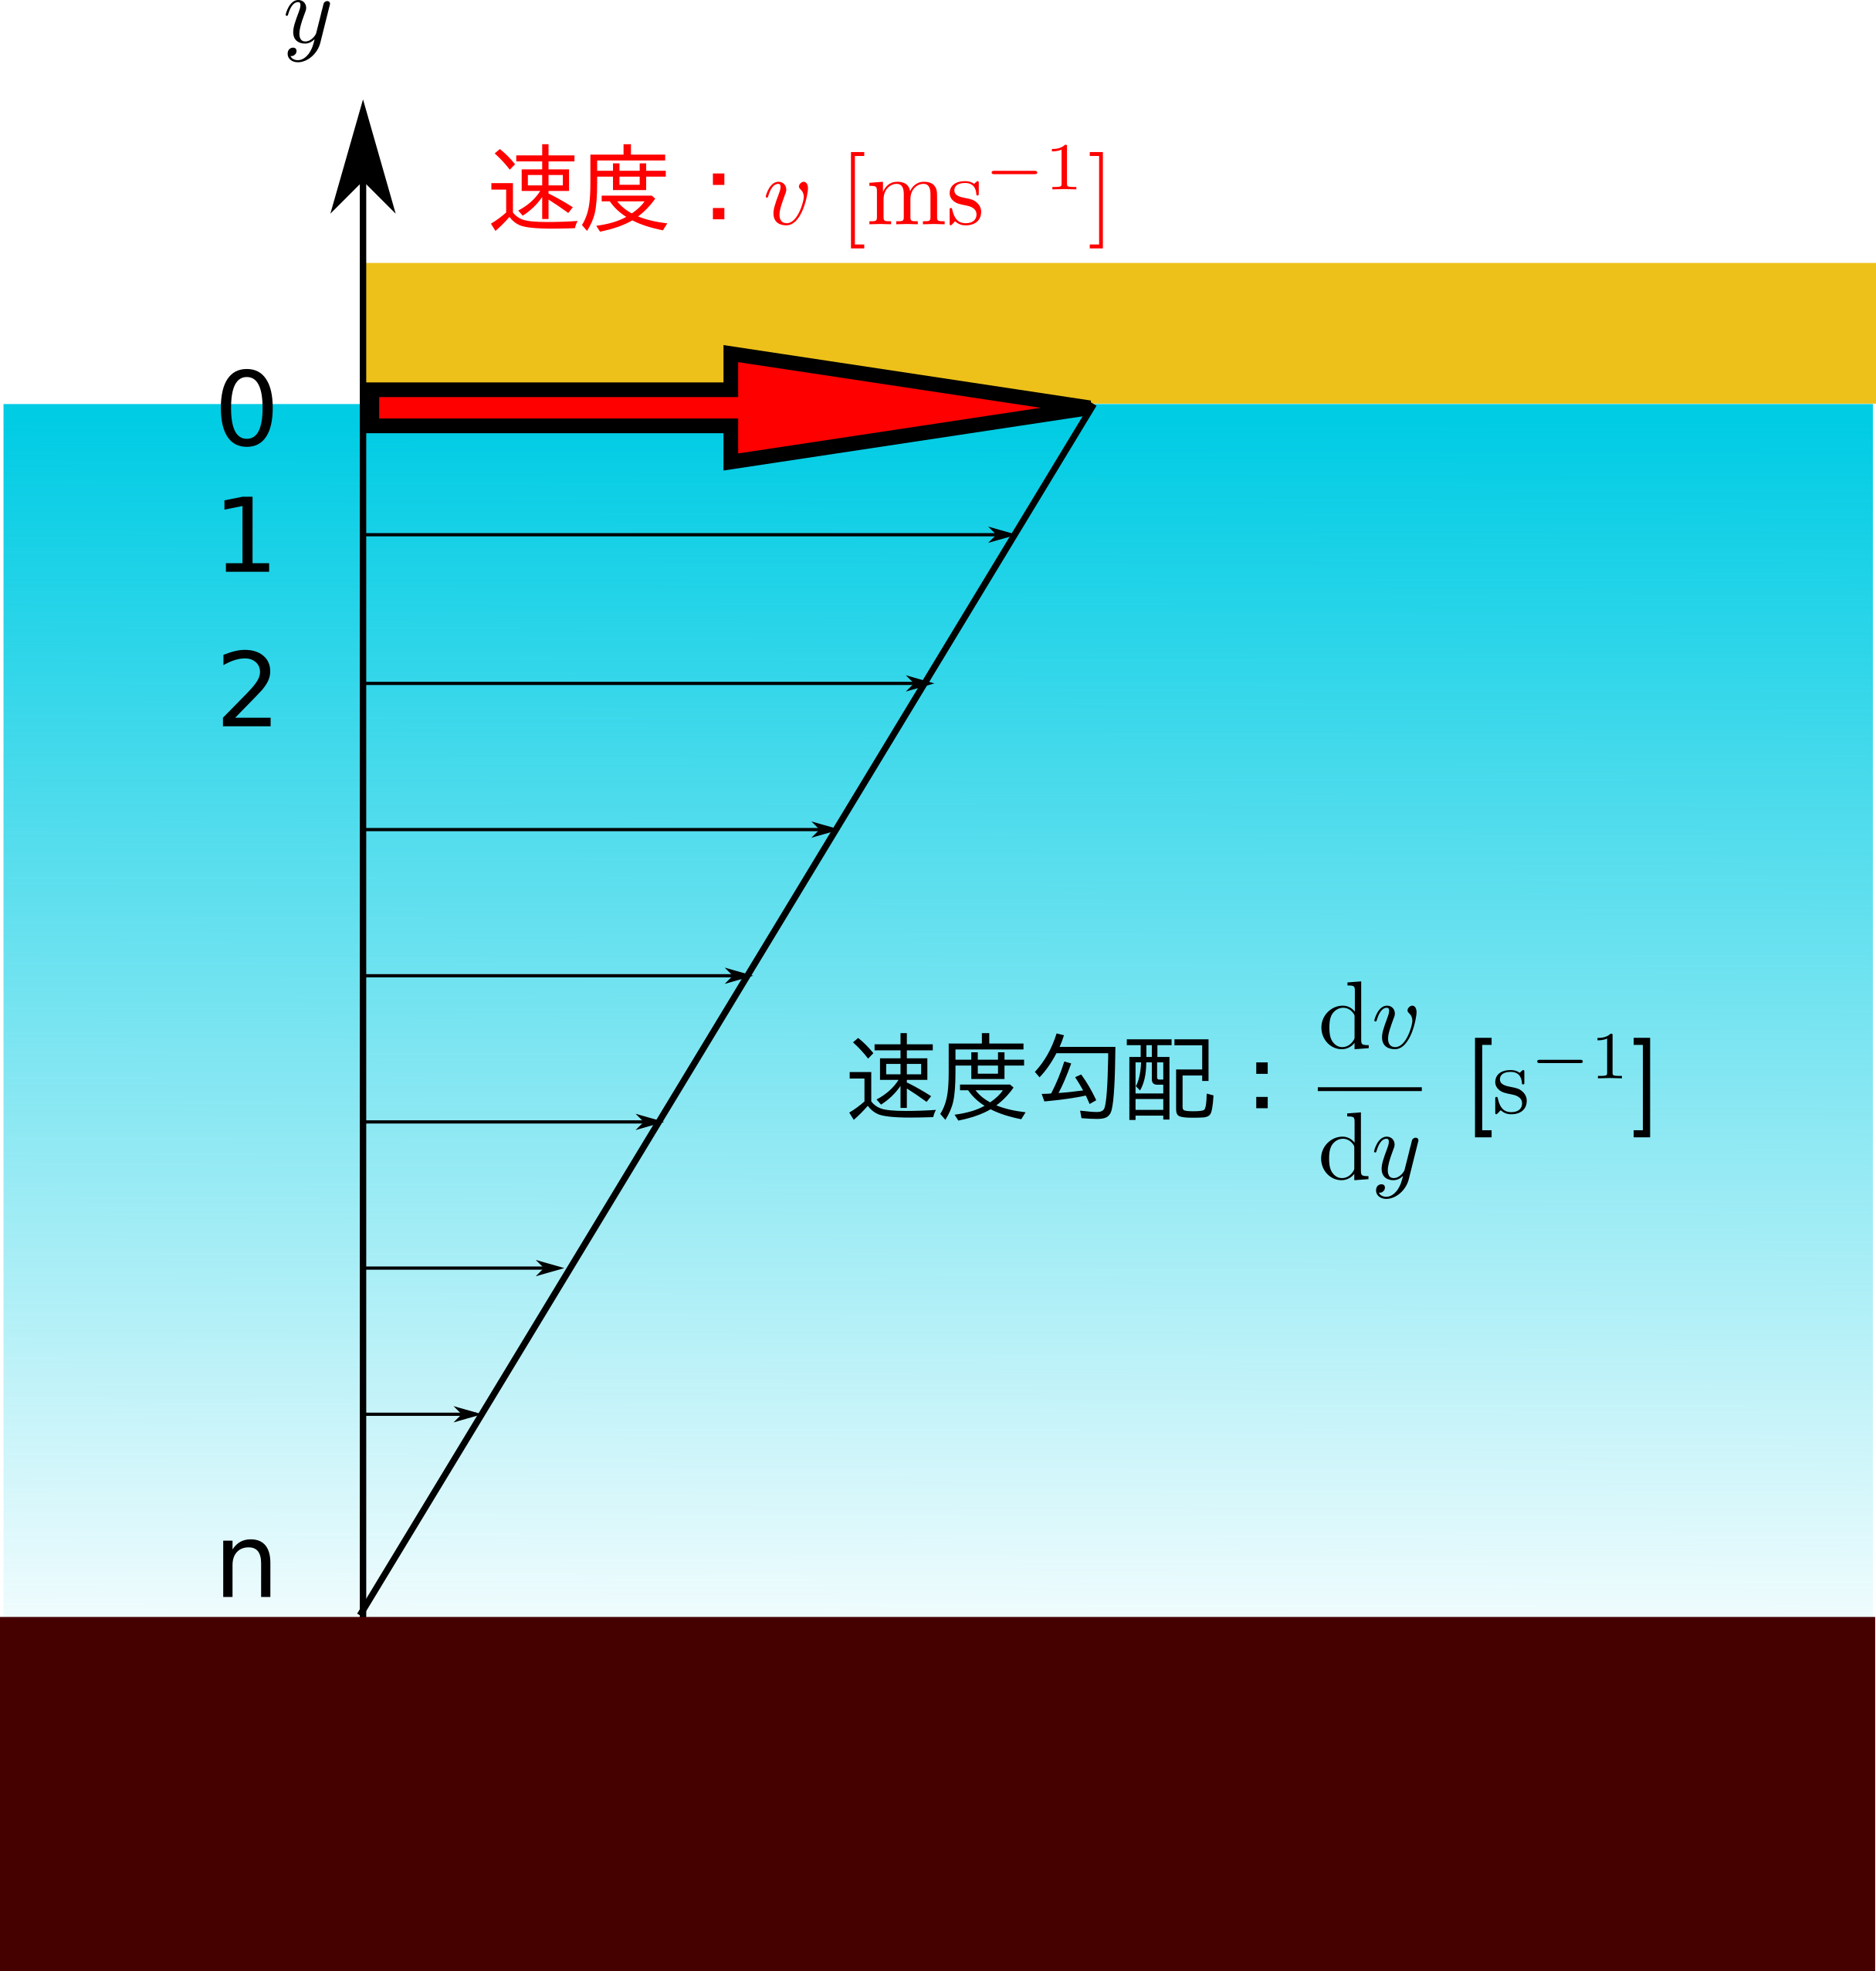
\includegraphics[width=.7\textwidth]{shear_3.png}
			\end{center}
		\end{minipage}
		\begin{minipage}{0.9\textwidth}
			\begin{center}
			\begin{itembox}[l]{注意すべきポイント}
				\begin{itemize}
					\item 固体と接している液体は、\textcolor{red}{その相対的な移動速度が同じ。}
					\begin{itemize}
						\item 移動する板と接している層 0 は板と同じ速度 $v$ で流れ、
						\item 地面に接している層 $n$ は流れない。
					\end{itemize}
					\item 評価の対象である液体の内部では、
					\begin{itemize}
						\item 水深に応じて、\textcolor{red}{流れる速度の分布が生じる。}
					\end{itemize}
					\item 液体の流れる速度は、
					\begin{itemize}
						\item 水深 $y$ の関数として $v(y)$
						\item \textcolor{red}{速度勾配と呼ばれ、その単位は $[\mathrm{s^{-1}}]$}
					\end{itemize}
				\end{itemize}
			\end{itembox}
			\end{center}
		\end{minipage}
		\caption{液体の流動のモデル}
		\label{fig:ryudo_model}
	\end{center}
\end{figure}


式 \eqref{eq:newton} に示した、ニュートン流体の式においては、上記のモデルで示したように、速度分布の勾配が一定になっている
最も単純な場合と考えることができます。

これらの事項を全部考慮して、結局、液体の力学モデルは図 \ref{fig:ryudo_model2} に示したように書くことができます。。
繰り返しになりますが、この速度勾配が傾き一定の定数になっていなければ、その液体はニュートン流動をしないということになります。

\begin{figure}[htb]
	\begin{center}
		\begin{minipage}{0.45\textwidth}
			\begin{itemize}
				\item せん断速度$\dot{\gamma}$ に比例し、
				\item せん断応力 $\tau$ が生じ、
				\item 比例定数が粘度 $\eta$
			\end{itemize}
			\begin{center}
				\begin{screen}
					\begin{center}
						上記の比例関係が成立する液体が\\ニュートン流体
					\end{center}
				\end{screen}
			\end{center}
		\end{minipage}
		\begin{minipage}{0.45\textwidth}
			\begin{center}
			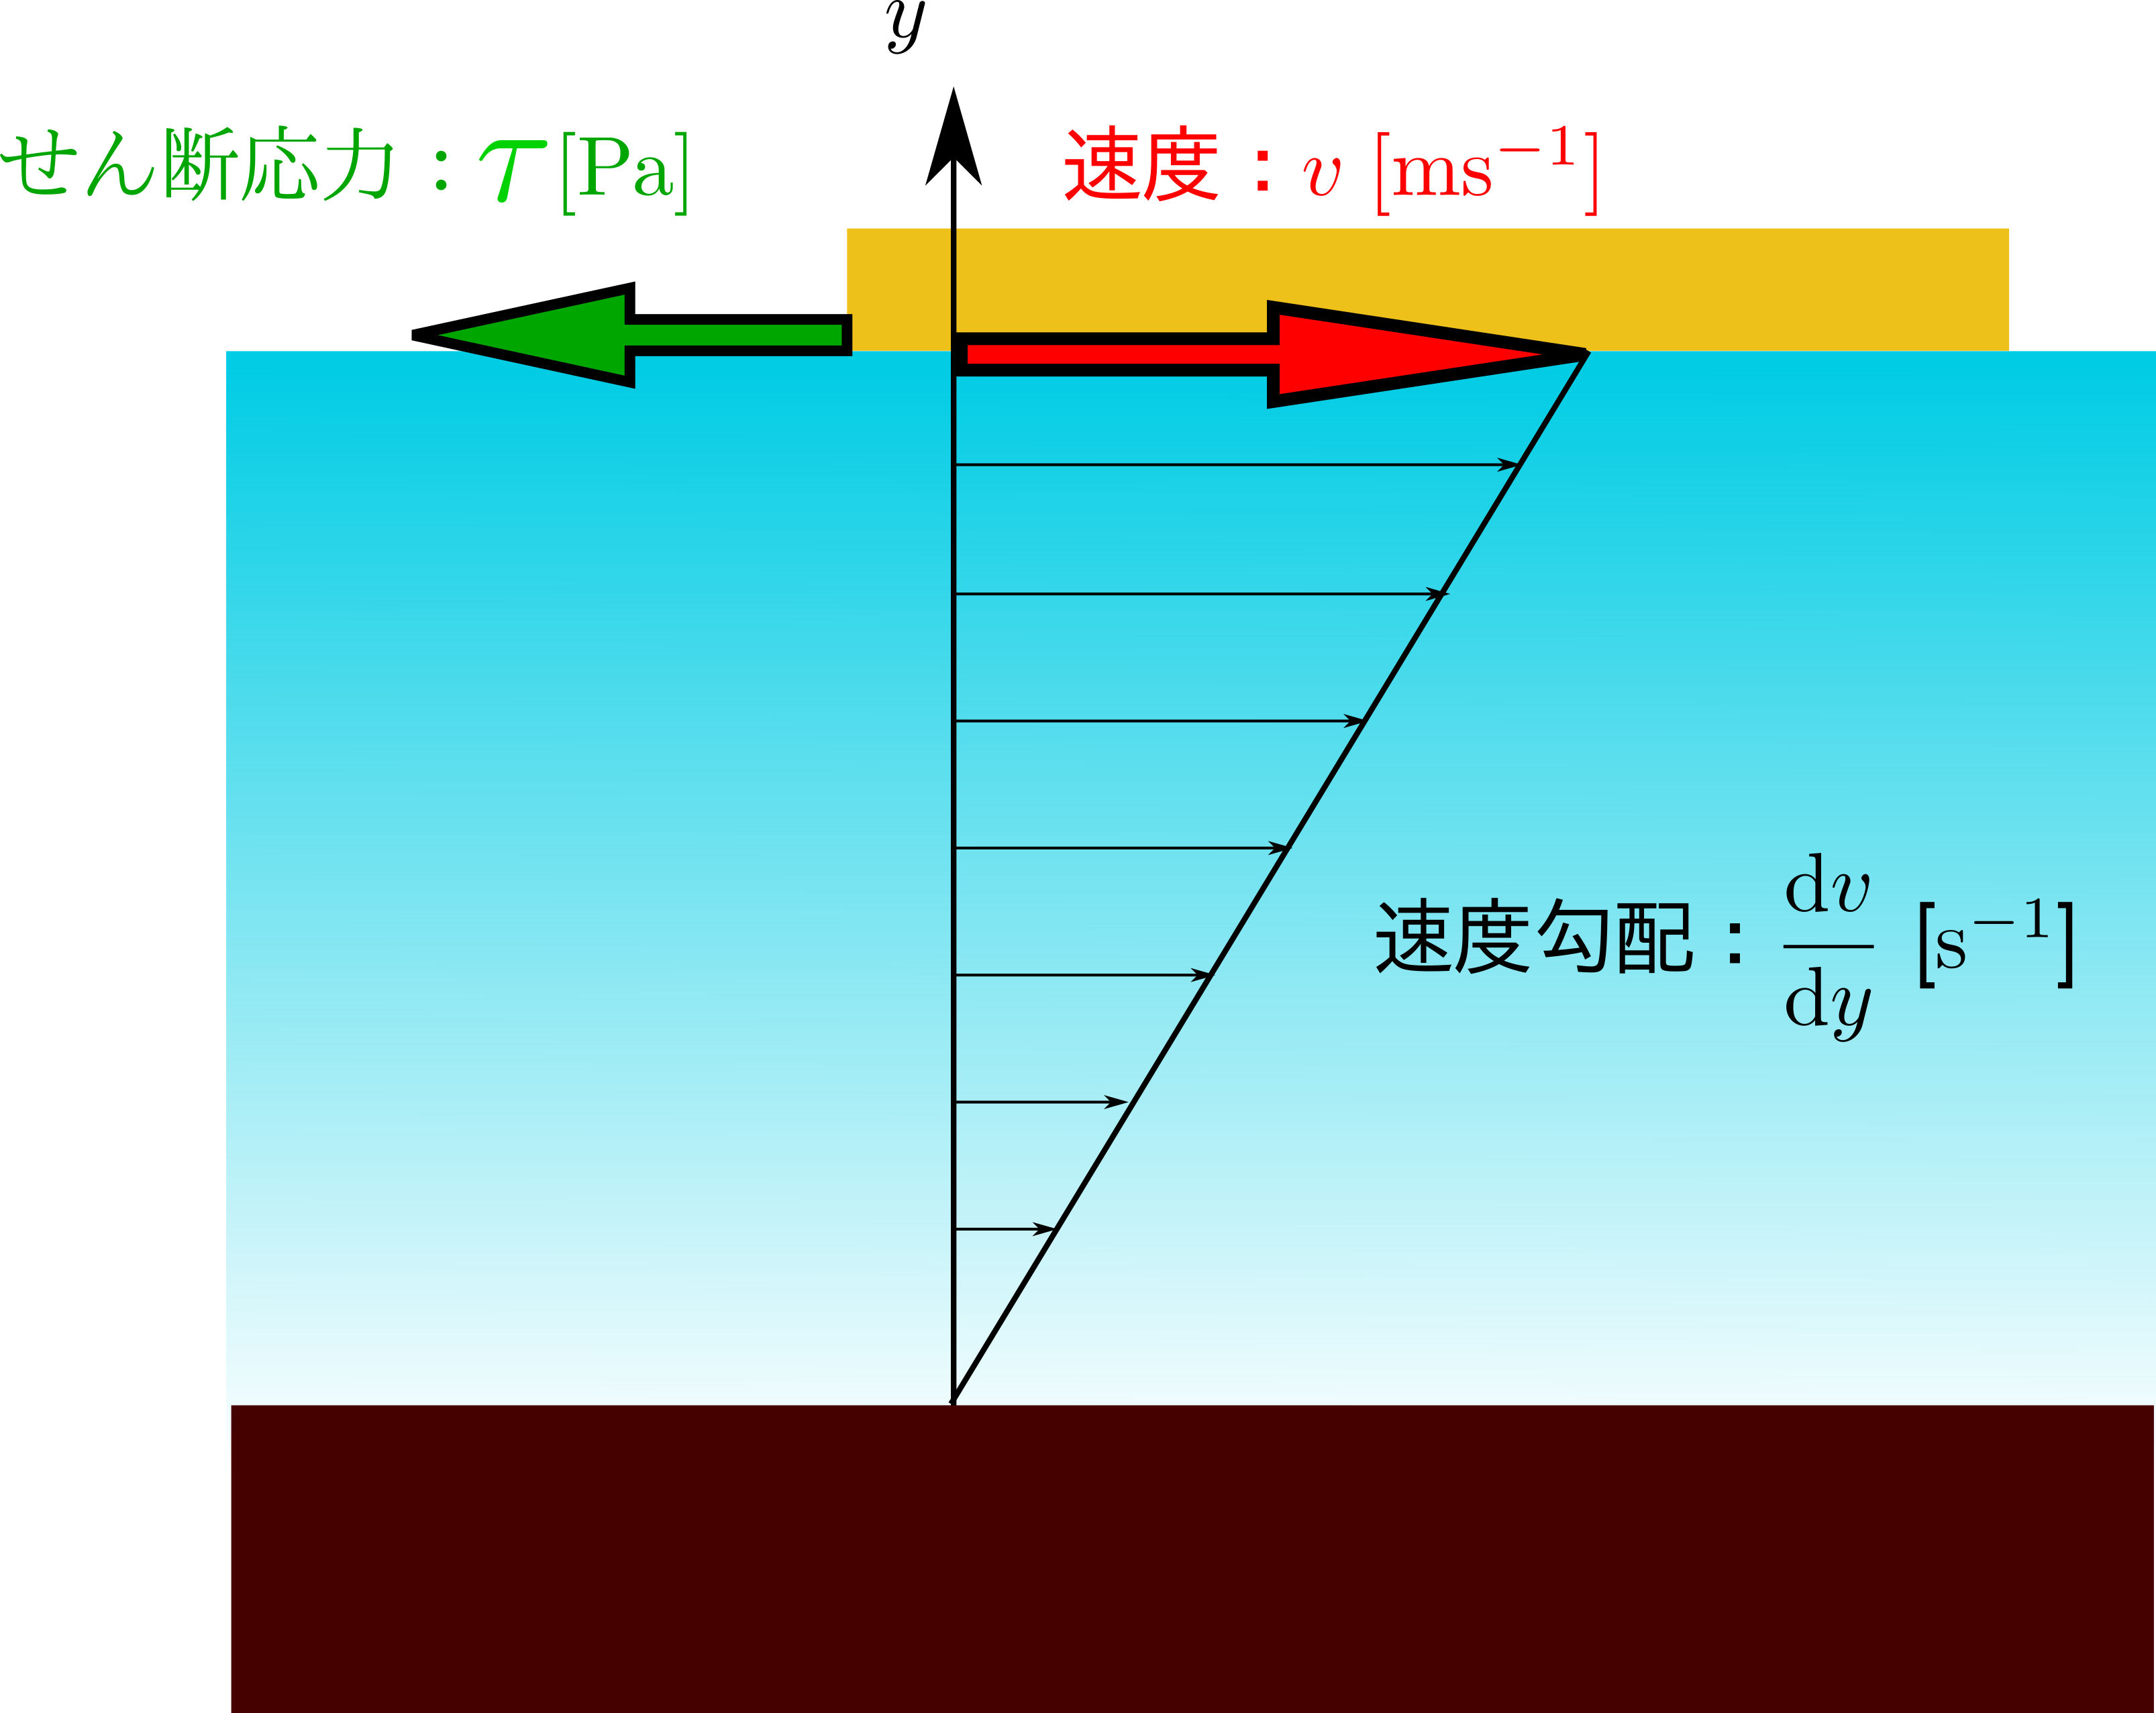
\includegraphics[width=.7\textwidth]{shear_4.png}
			\end{center}
		\end{minipage}
		\begin{minipage}{0.9\textwidth}
			\begin{center}
			\begin{itembox}[l]{ニュートン流体の特徴}
				\begin{itemize}
					\item 速度勾配に従って、各層ごとにせん断応力が発生
					\begin{itemize}
						\item その値は、\textcolor{red}{局所的なせん断速度に比例して変化。}
						\item 逆に言えば、\textcolor{red}{せん断速度によらずに粘度が一定。}
					\end{itemize}
				\end{itemize}
			\end{itembox}
			\end{center}
		\end{minipage}
		\caption{液体の力学モデルとニュートン流体}
		\label{fig:ryudo_model2}
	\end{center}
\end{figure}

\subsection{局所的な応力と粘度}

\subsubsection{ミクロに見た液体の流動のモデルを再び}

つぎに、このようなニュートン流動を示す液体のミクロな描像を考えてみましょう。

以前に示した、「液体の応力のミクロな描像」を図 \ref{fig:stress_micro} に再掲しました。
\begin{figure}[htb]
	\begin{center}
		\begin{minipage}{0.9\textwidth}
			\begin{center}
				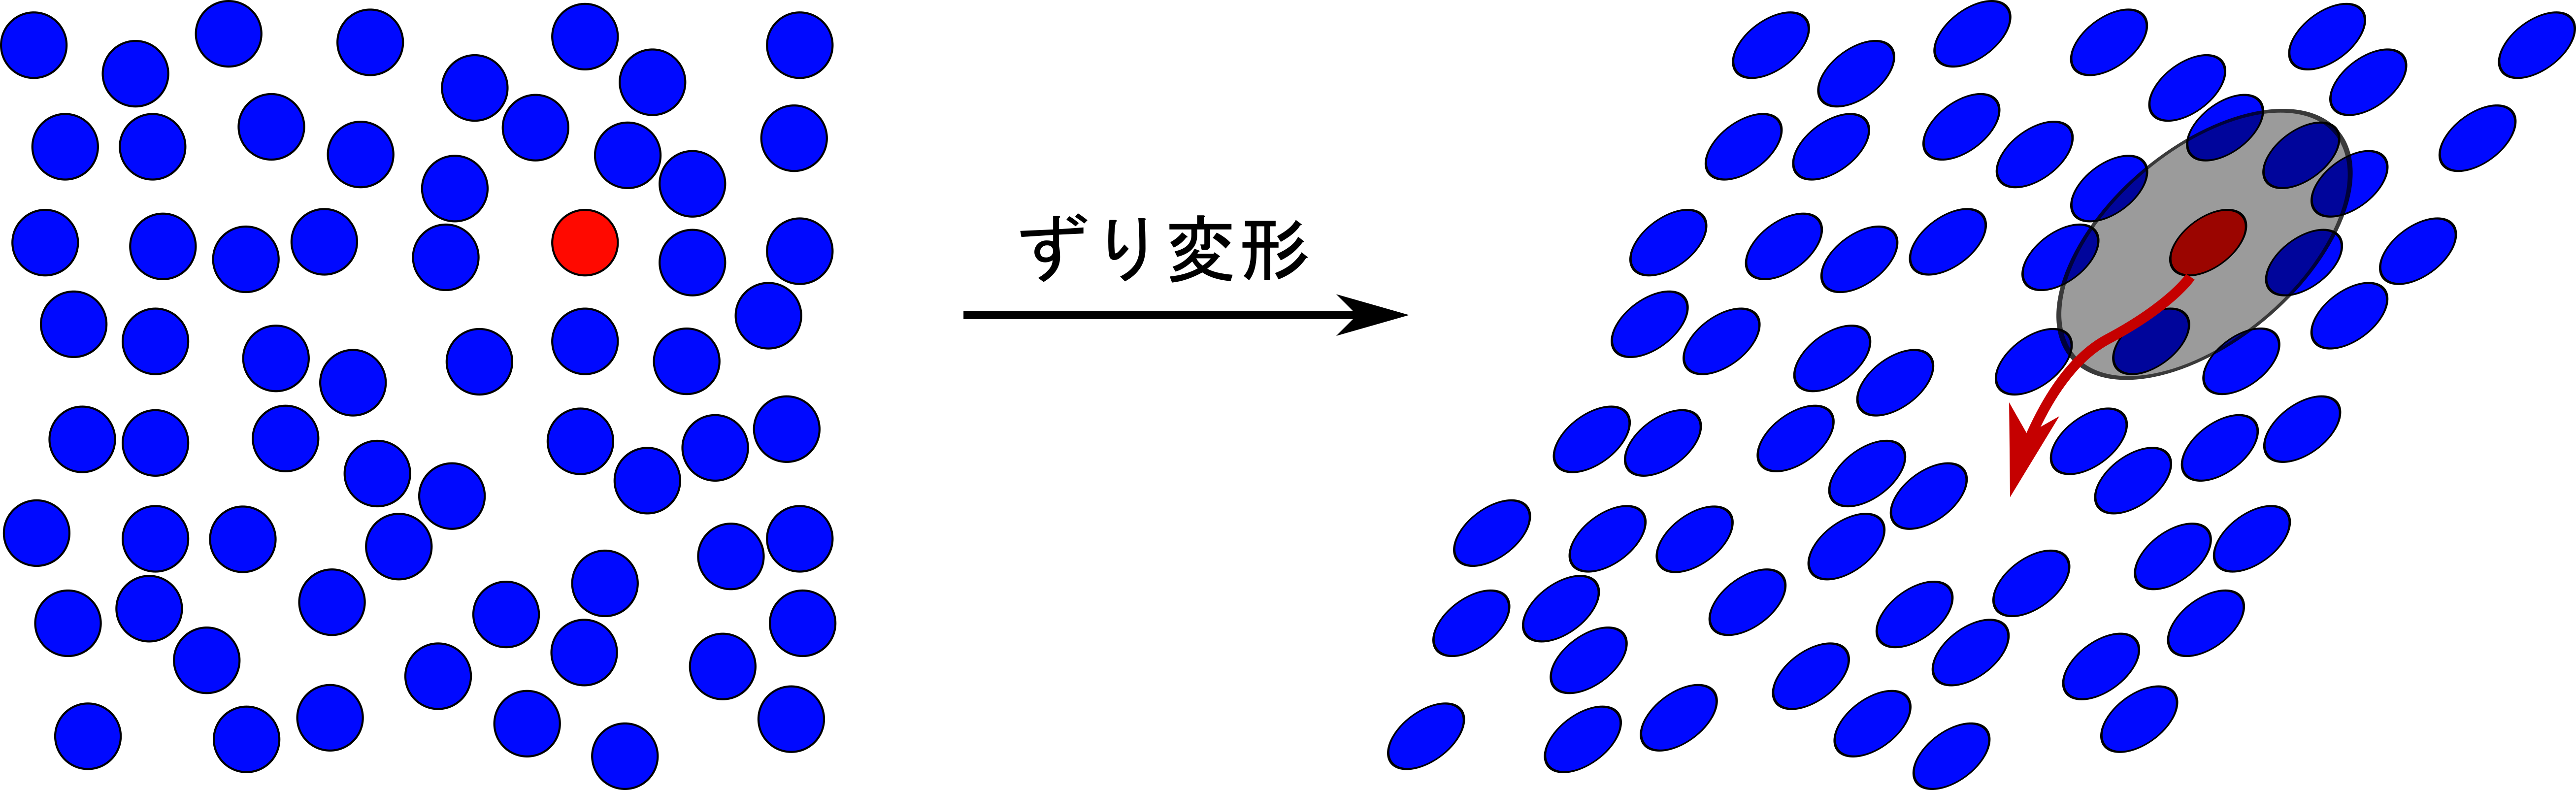
\includegraphics[width=.8\textwidth]{liquid_flow.png}
			\end{center}
		\end{minipage}
		\begin{minipage}{0.9\textwidth}
			\begin{center}
				\begin{itembox}[l]{液体の応力のミクロな表現}
					\begin{itemize}
						\item マクロな変形(例えば、せん断変形)を付与
						\begin{itemize}
							\item ミクロにも粒子近傍の並び方が変化
						\end{itemize}
						\item 一粒子に着目すると、
						\begin{itemize}
							\item その粒子を取り巻く周りの粒子とのポテンシャル場が変化して、\textcolor{red}{「歪んだかご」}
							\item 「歪んだかご」の中で、\textcolor{red}{居心地が悪くなる。}
							\item その結果として\textcolor{red}{局所的な応力が発現}
						\end{itemize}
						\item その積分値として、マクロな応力
						\begin{itemize}
							\item 「歪んだかご」からの\textcolor{red}{脱出 $\Leftrightarrow$ ミクロな応力が消失 }
							\item マクロにも\textcolor{red}{流動}
						\end{itemize}
					\end{itemize}
				\end{itembox}
			\end{center}
		\end{minipage}
		\caption{液体の応力のミクロな描像}
		\label{fig:stress_micro}
	\end{center}
\end{figure}

マクロな変形が付与されたとき、ミクロな環境においても粒子近傍の並び方は変化するのでした。

このとき、一粒子に着目すると、その粒子を取り巻く周りの粒子とのポテンシャル場が変化してしまい、「歪んだかご」の中にとらわれているようになります。
そして、「歪んだかご」の中で、居心地が悪くなった結果として局所的な応力が発現し、その積分値として、マクロな応力が生じます。
さらに、その注目する粒子が「歪んだかご」から脱出すれば、ミクロな応力が消失してマクロな流動が生じていると考えてきました。

これは、マクロな変形による流動は、流体の構成要素である粒子が局所的な場における居心地の悪さから脱出することによって
生じていると考えるモデルです。

\subsubsection{液体のメゾスケールのモデルと合わせると}
では、上記のようなミクロの描像のモデルと、液体を仮想的に層状に分割してその速度勾配を考えた、中間的な大きさを表すメゾスケールモデルとの
整合性を考えてみましょう。
\begin{figure}[htb]
	\begin{center}
		\begin{minipage}{0.52\textwidth}
			\begin{itembox}[l]{せん断応力の由来}
				\begin{itemize}
					\item 仮想的な面で生じるせん断応力の由来は、
					\begin{itemize}
						\item \textcolor{red}{面を通しての粒子の相互作用}に起因
						\item 相対的な速度差に、比例する
					\end{itemize}
					\item この相互作用は、
					\begin{itemize}
						\item 「歪んだかご」からの脱出頻度にも比例
						\item 多体の相互作用が、「居心地の悪さ」
					\end{itemize}
				\end{itemize}
			\end{itembox}
		\end{minipage}
		\begin{minipage}{0.4\textwidth}
			\begin{center}
			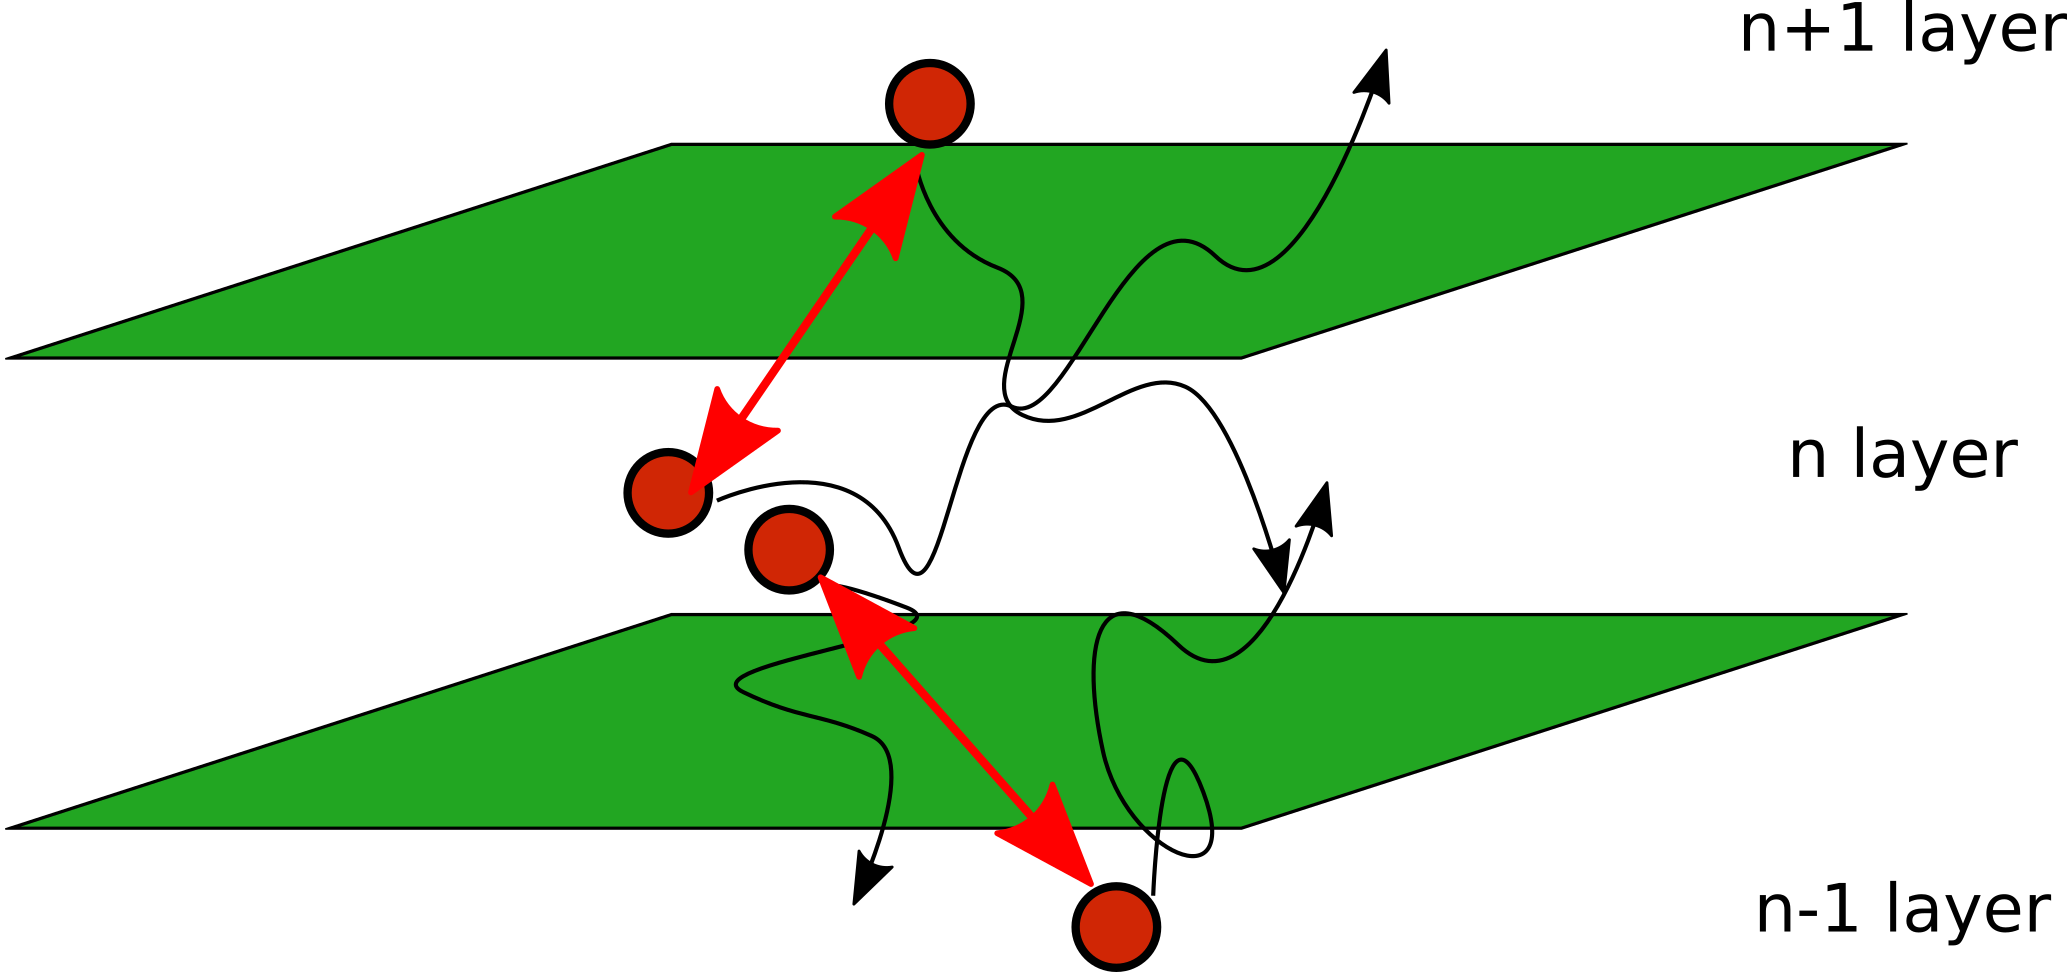
\includegraphics[width=\textwidth]{flow_layer.png}
			\end{center}
		\end{minipage}
		\caption{せん断応力の由来}
		\label{fig:origin_stress}
	\end{center}
\end{figure}

ミクロな粒子のかごからの脱出と、層ごとの流れをメゾスケールで考えることを同時に行うと、
仮想的に分割した層同士の接した面で生じるせん断応力の由来は、面を通しての粒子の相互作用に起因すると考えることができます。
そして、層同士の相対的な速度差に比例して、ミクロに見たときの「かごの歪具合」、すなわち、「居心地の悪さ」が変化するので、
粒子の脱出頻度もその環境に応じて変化すると考えるわけです。

\subsubsection{結局、ニュートン流体とは}

ここまで示してきたメゾスケールでの仮想的な層ごとの速度を考えるモデルと、
ミクロスケールでの粒子の居心地を想定したモデルとを合わせて考えてみましょう。
ニュートン流体においては、隣接する粒子間の相互作用がマクロなせん断速度やせん断応力に依存しないと考えられ、
その結果として、マクロな粘度が一定になっているものと捉えることができます。

\begin{figure}[htb]
	\begin{center}
		\begin{minipage}{0.9\textwidth}
			\begin{itembox}[l]{ニュートン流体では}
				\begin{itemize}
					\item 隣接する粒子間の相互作用が、\textcolor{red}{せん断速度やせん断応力に非依存。}
					\item 結果、粘度が一定。
					\item ただし、\textcolor{red}{変形速度が適正な範囲で成立。}
				\end{itemize}
			\end{itembox}
		\end{minipage}
	\end{center}
\end{figure}

逆に言えば、そのような状態が成立しなくなってくると、線形な応答であるニュートン流動は見られなくなると考えることができます。

\subsubsection{粒子が共存した場合}

ニュートン流体に球状粒子が入った場合については、あの有名なアインシュタインが理論的に導出しています。
具体的には、剛直な球を希薄に懸濁した溶液を想定して、以下のような仮定条件を定めて議論しています。
\begin{itemize}
	\item 球の半径は、液体粒子より遥かに大きい。
	\item 球状粒子間の相互作用はない。
	\item 液体粒子は球状粒子に固着している。
\end{itemize}

このような条件が成り立つのであれば、ニュートン流動の特徴である線形性を維持しながら濃度が上昇することになります。

アインシュタインは、砂糖水の濃度と粘度との関係から、下式を使って砂糖分子の大きさと分子数を概算しています。
\begin{align*}
	&\eta = \eta_0(1+2.5\phi) \\
	&\text{\small $\eta_0$は液体の粘度、$\phi$ は球状粒子の体積分率}
\end{align*}

この導出の過程においては、以下のように考えているようですが、詳細は難解ですので省略します。
\begin{figure}[htb]
	\begin{center}
		\begin{minipage}{0.9\textwidth}
			\begin{center}
			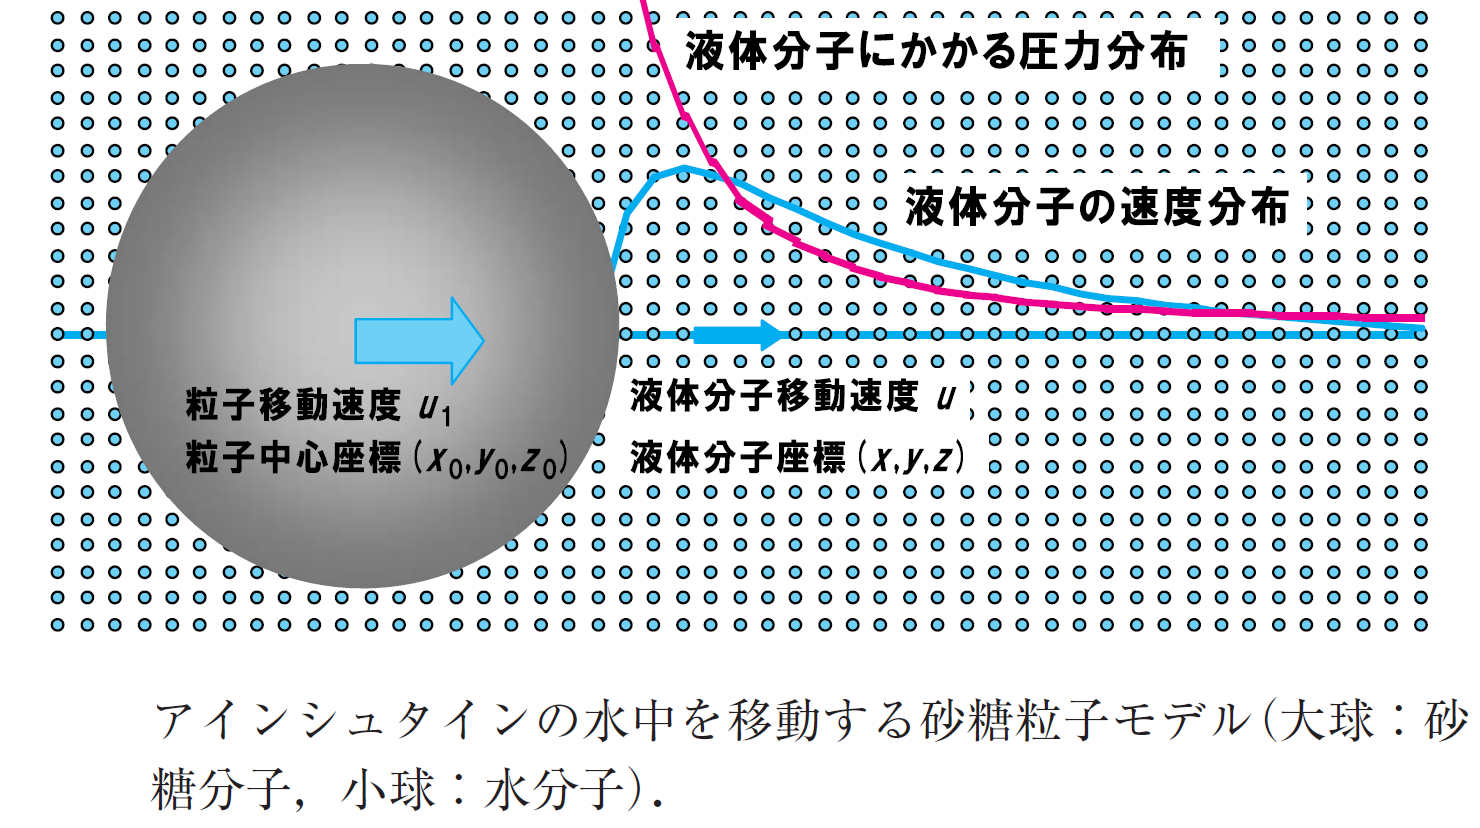
\includegraphics[width=.8\textwidth]{Einstein.png}
			\end{center}
		\end{minipage}
		\begin{minipage}{0.9\textwidth}
			\begin{enumerate}
				\item すべての水分子の水平変位は、その相対位置を保ちながら起こる。
				\item 水分子の回転は、その相対位置を保ちながら起こる。
				\item 水の膨張・収縮は三次元で起こる。
			\end{enumerate}
		\end{minipage}
		\caption{アインシュタインのモデルについて}
		\label{fig:einshtain}
	\end{center}
\end{figure}



\section{非ニュートン流体について}
\subsection{身近な液体とその分類}
ここでは、身近な液体について振り返ることで、実際には非ニュートン流体が多いことを再確認していきましょう。
\begin{figure}[htb]
	\begin{center}
		\begin{minipage}{0.45\textwidth}
			\begin{center}
			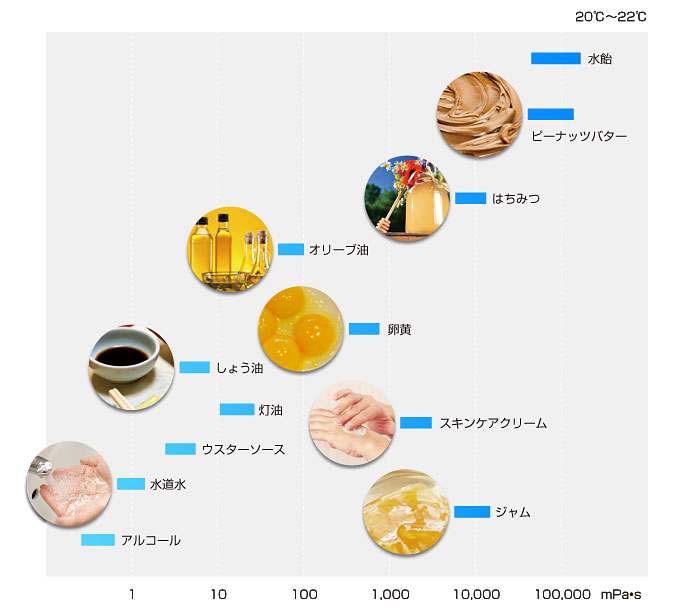
\includegraphics[width=.8\textwidth]{viscosity.jpg}
			\end{center}
		\end{minipage}
		\begin{minipage}{0.45\textwidth}
			\begin{itembox}[l]{身近な液体の粘度}
				\begin{itemize}
					\item 一般的には左図のように、流れやすさを一覧に表す。
					\item 一応は、粘度の順番で並べて比較している。
					\item それで十分なのだろうか?
					\item \textcolor{red}{実は、測り方によっては順位は前後する場合も多い。}
				\end{itemize}
			\end{itembox}
		\end{minipage}
		\caption{身の回りにある各種の液体の粘度}
	\end{center}
\end{figure}

一般的には、流れやすさを粘度という数値で捉えて、数字の大きさで流れやすさを比較しています。
でも、本当にそんなに単純に流れやすさを比べることができるのでしょうか。
実は、測り方によっては流れやすさの順位が前後する場合も多いのです。

また、それぞれの物質ごとに流れ方も大きく異なってくることがよく知られています。
以前に示した、ビンガム氏が作成した流動特性の分類図を、再度よく見てみましょう。
\begin{figure}[htb]
	\begin{center}
		\begin{minipage}{0.9\textwidth}
			\begin{itemize}
				\item 図の左側が固体的な弾性応答を表していて、右側が液体的な流動特性を示している。
				\item ここに記されたように、固体と液体に単純に二分されるわけでもなく、
				粘性と弾性を併せ持ったものが多く存在することがわかる。
			\end{itemize}
		\end{minipage}
		\begin{minipage}{0.9\textwidth}
			\begin{center}
			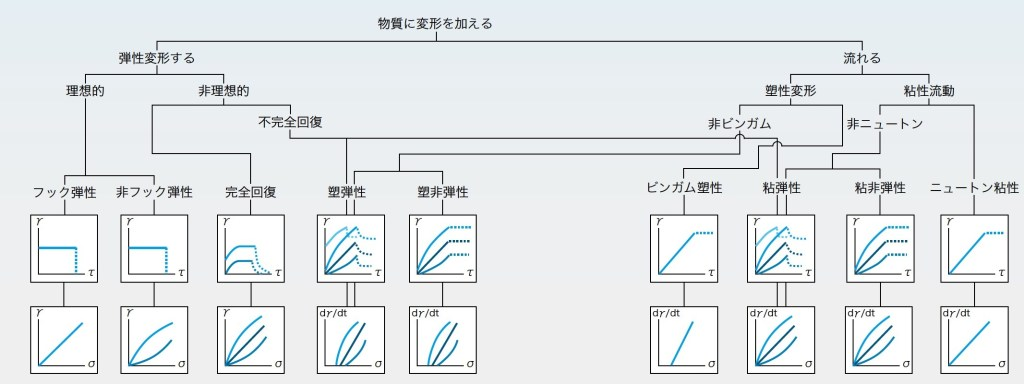
\includegraphics[width=\textwidth]{reoroji.jpeg}

			Nature 1942 v149-3790, p702
			\end{center}
		\end{minipage}
		\caption{ビンガム氏が作成した流動特性の分類図}
	\end{center}
\end{figure}

\subsection{非ニュートン流体とは}

非ニュートン流体を簡単に定義すると、ニュートン流動と異なる流動特性を示すもの全部ということになります。
\begin{itemize}
	\item せん断速度とせん断応力との関係が線形ではない。
	\item 変形状態(せん断速度や加える力が変化)に依存して、粘度が変化する。
\end{itemize}

そのような流動特性を示す原因は多数ありますが、基本的に内部に構造を有する物質で多くの場合生じる事が知られています。
なお、具体的な内容については、次の節で説明を行います。

\begin{figure}[htb]
	\begin{center}
		\begin{minipage}{0.9\textwidth}
			\begin{itembox}[l]{非ニュートン流体とは?}
				\begin{itemize}
					\item 簡単に言えば、ニュートン流動と異なる流動特性を示すもの。
					\begin{itemize}
						\item せん断応力が線形ではない。
						\item 変形状態(せん断速度や加える力が変化)に依存して、粘度が変化する。
					\end{itemize}
					\item その原因は多数あるが、基本的に内部に構造を有する物質で生じる。
				\end{itemize}
			\end{itembox}
		\end{minipage}
		\begin{minipage}{0.45\textwidth}
			\begin{center}
			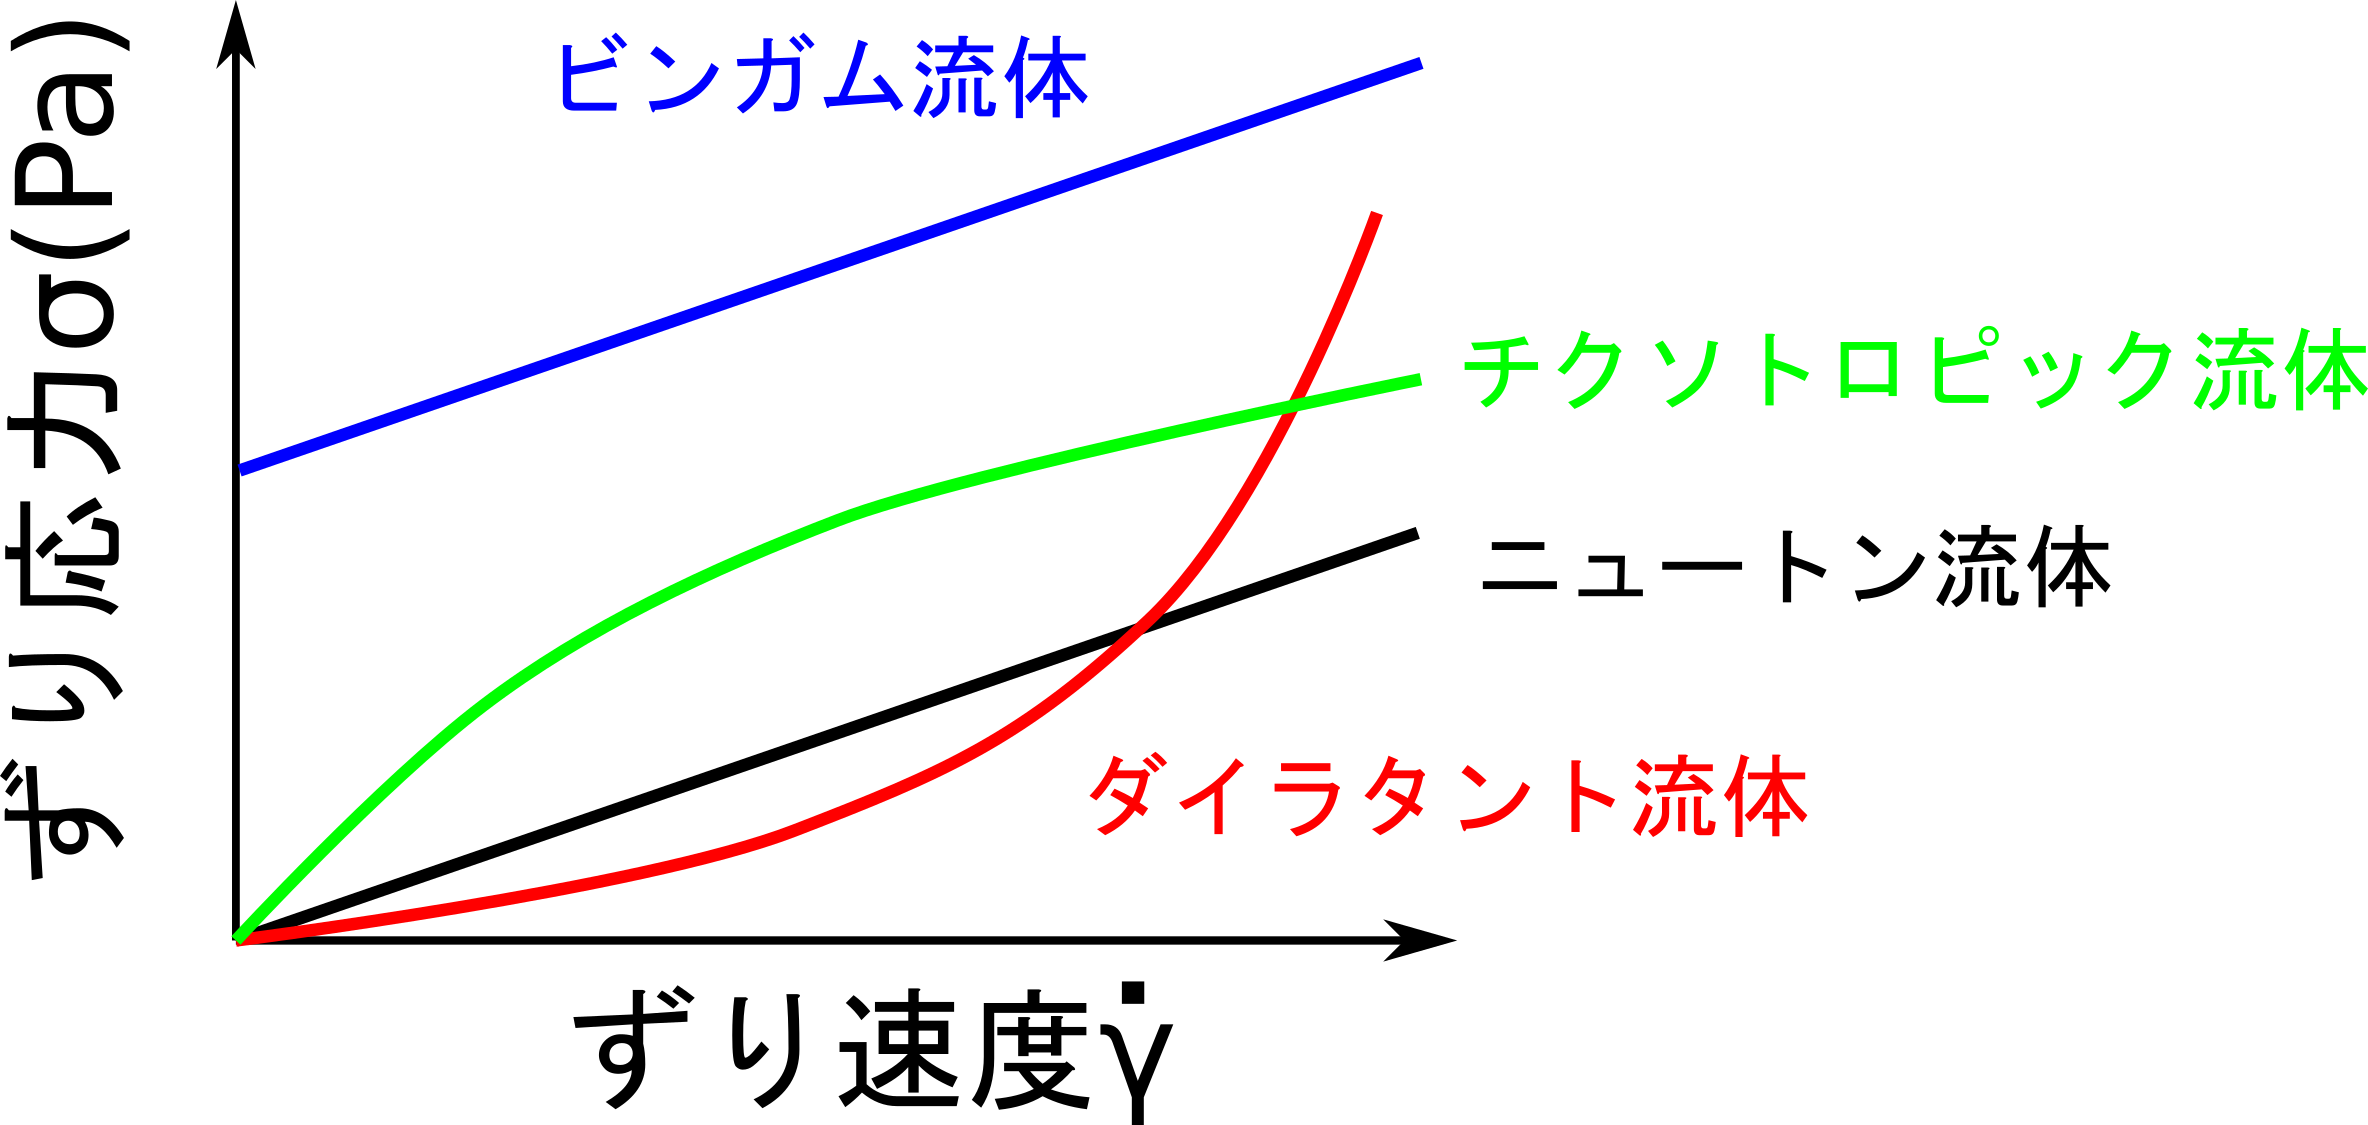
\includegraphics[width=\textwidth]{non_newtonian.png}
			\end{center}
		\end{minipage}
		\begin{minipage}{0.45\textwidth}
			\begin{center}
			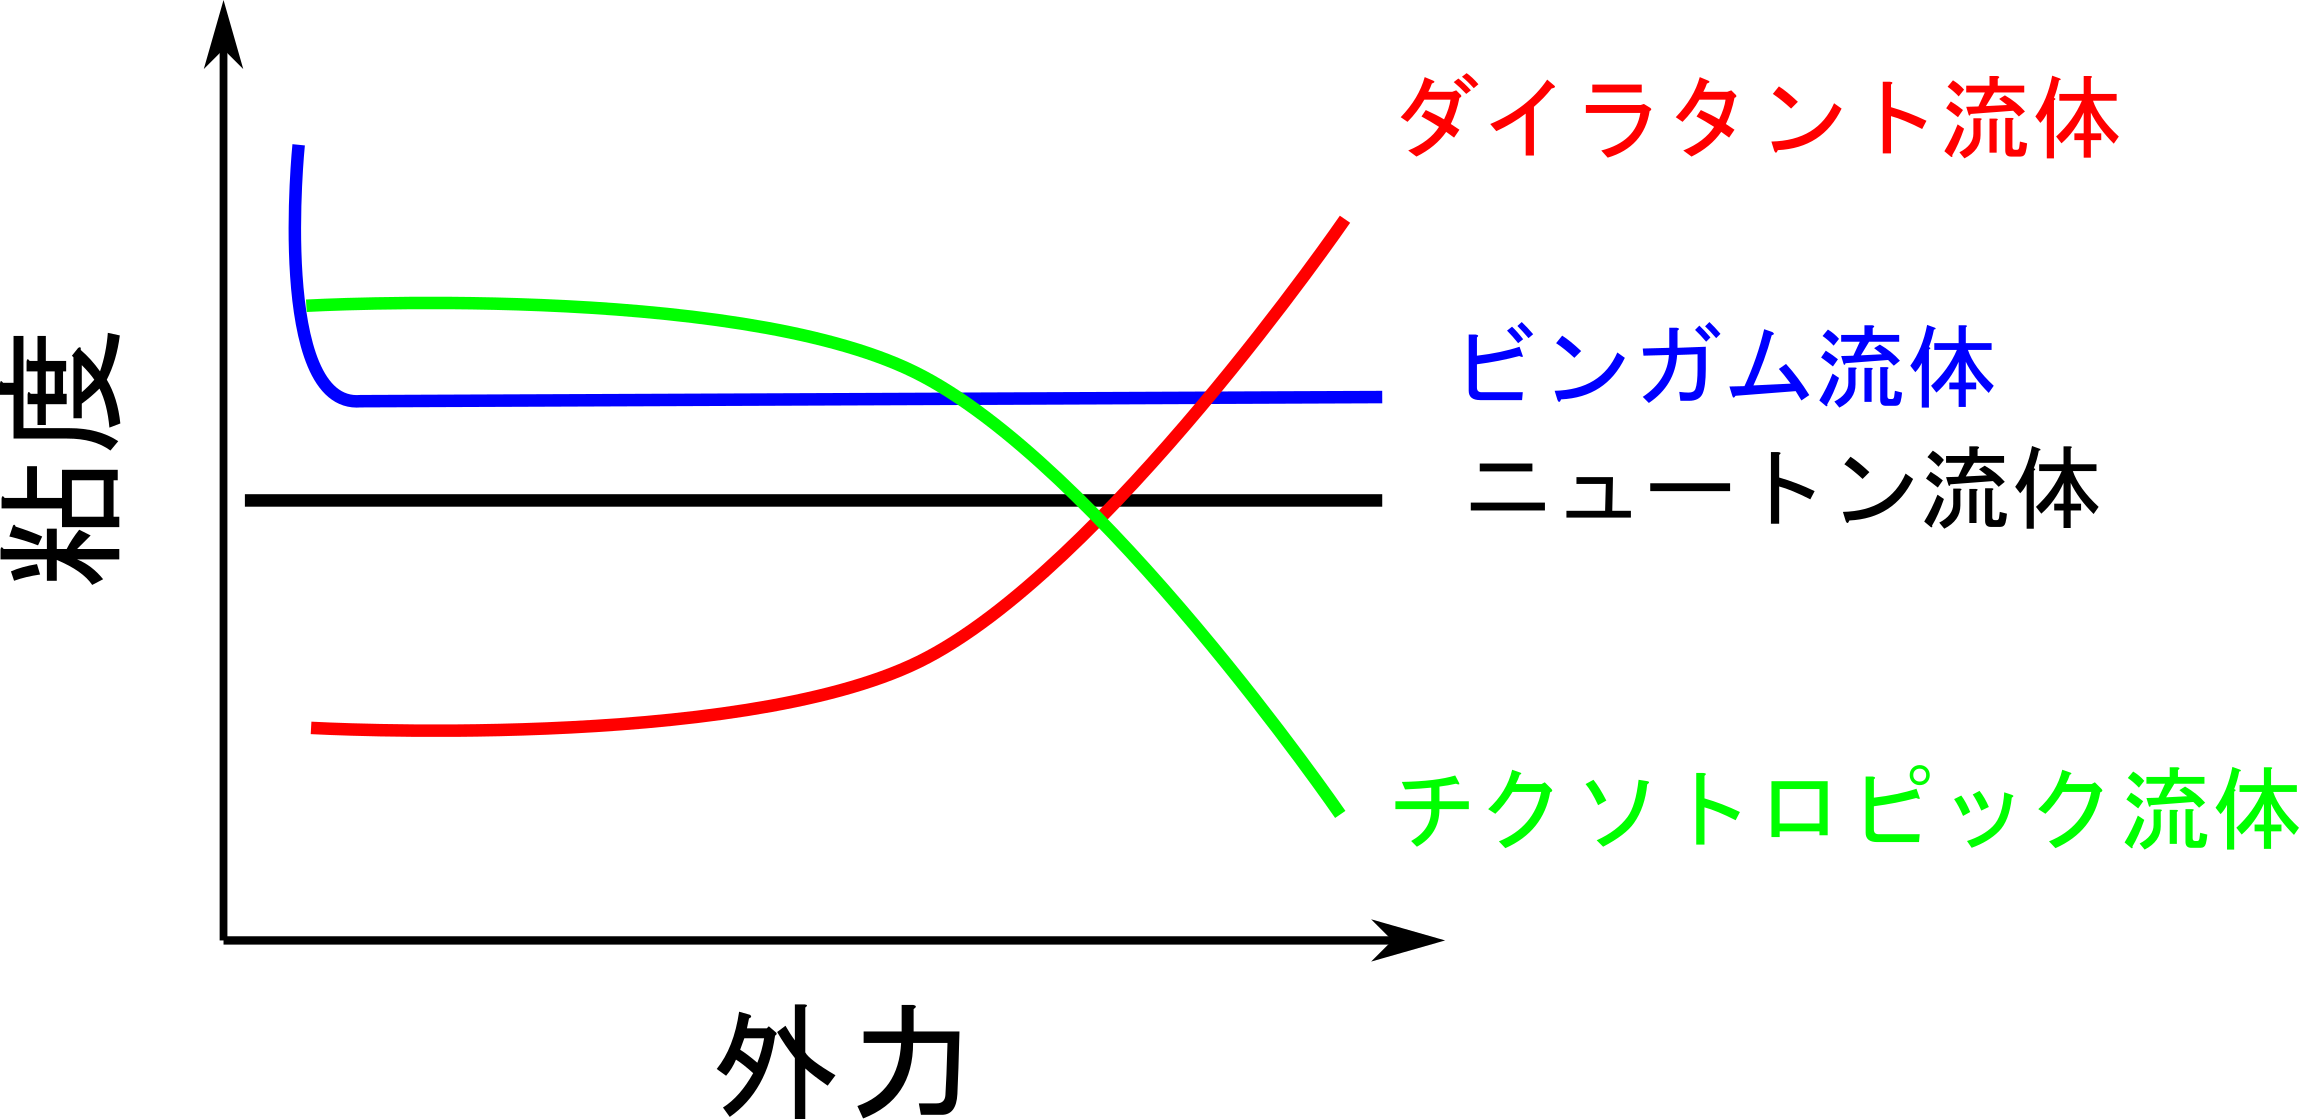
\includegraphics[width=\textwidth]{non_newtonian_2.png}
			\end{center}
		\end{minipage}
		\caption{非ニュートン流体とは}
		\label{fig:non_newtonian}
	\end{center}
\end{figure}

\subsection{非ニュートン性の発現}
\subsubsection{非ニュートン性の直感的理解}
流動特性の非線形性について、直感的な理解を目指しましょう。

様々な物質の流動特性は、物質の内部構造に由来して応力(粘度)が、増加したり、減少したりすることに起因しています。
このとき、以下のように、系の挙動を支配する特徴的な時間が存在すると考えてみましょう。
\begin{itembox}[l]{系の挙動を支配する特徴的な時間}
	\begin{itemize}
		\item 物質の内部構造に由来する特徴的時間が存在し、
		\item これは、内部構造が崩壊、再構築するための特徴的な時間と考える。
	\end{itemize}
\end{itembox}

そのとき、外部からの変形に関わる時間(変形に関与する時間)と、この系固有の特徴的な時間との比が大事になってくるわけです。
すなわち、物質中の内部構造が持つ特徴的な時間よりも短い時間(速い速度)で変形しようとすると、非ニュートン性が発現すると考えることができます。
\begin{itembox}[l]{非ニュートン性の発現}
	\begin{itemize}
		\item 内部構造が変化するため巨視的な粘度が変化し、
		\item \textcolor{red}{非ニュートン性が発現する。}
	\end{itemize}
\end{itembox}

一方、内部の特徴時間よりゆっくり変形した場合には、その範囲では、粘度は変形速度に依存しないことになり、
線形として応答してニュートン流動特性を示すと考えることができます。

\subsubsection{様々な事象のせん断速度}
以下に様々な工程における大体のせん断速度の範囲を、簡単にまとめました。
外部からの変形が異なってきた場合に、対象となる物質の持つ特徴的な時間との関係に応じて非ニュートン性が発現してくることになります。

\begin{table}[htb]
	\caption{様々な事象のせん断速度}
	\begin{center}
		\begin{tabular}{c|c} \hline
			工程 & せん断速度 \\ \hline \hline
			粒子の沈降	& $10^{-6} \sim 10^{-3}$ \\ \hline
			表面張力によるレベリング	& $10^{-2} \sim 10^{-1}$ \\ \hline
			重力による液垂れ	& $10^{-1} \sim 10^{1}$ \\ \hline \hline
			押し出し	& $10^{0} \sim 10^{3}$ \\ \hline
			ボトルからの流れ出し	& $10^{1} \sim 10^{2}$ \\ \hline
			噛む、飲む	& $10^{1} \sim 10^{2}$ \\ \hline
			混合攪拌	& $10^{1} \sim 10^{3}$ \\ \hline
			塗工	& $10^{0} \sim 10^{4}$ \\ \hline
		\end{tabular}
	\end{center}
\end{table}


\section{実事象についても少しだけ考えましょう。}
\subsection{簡単な分類}

ひずみ速度を変化させた場合の、粘度やせん断応力の依存性について簡単に分類すると、図 \ref{fig:shearrate_dep} に示したように、
粘度が上昇するものをシア・シックニングと呼び、ダイラタント流体をその例としてあげることができます。
一方、低下するものをシア・シニングとして、チクソトロピック流体が典型的な例となります。

なお、このような記述において、粘度がせん断速度に依存しないものがニュートン流体となりますが、
せん断速度が上がれば応力は増加することに注意してください。
\begin{figure}[htb]
	\begin{center}
		\begin{minipage}{0.45\textwidth}
			\begin{center}
			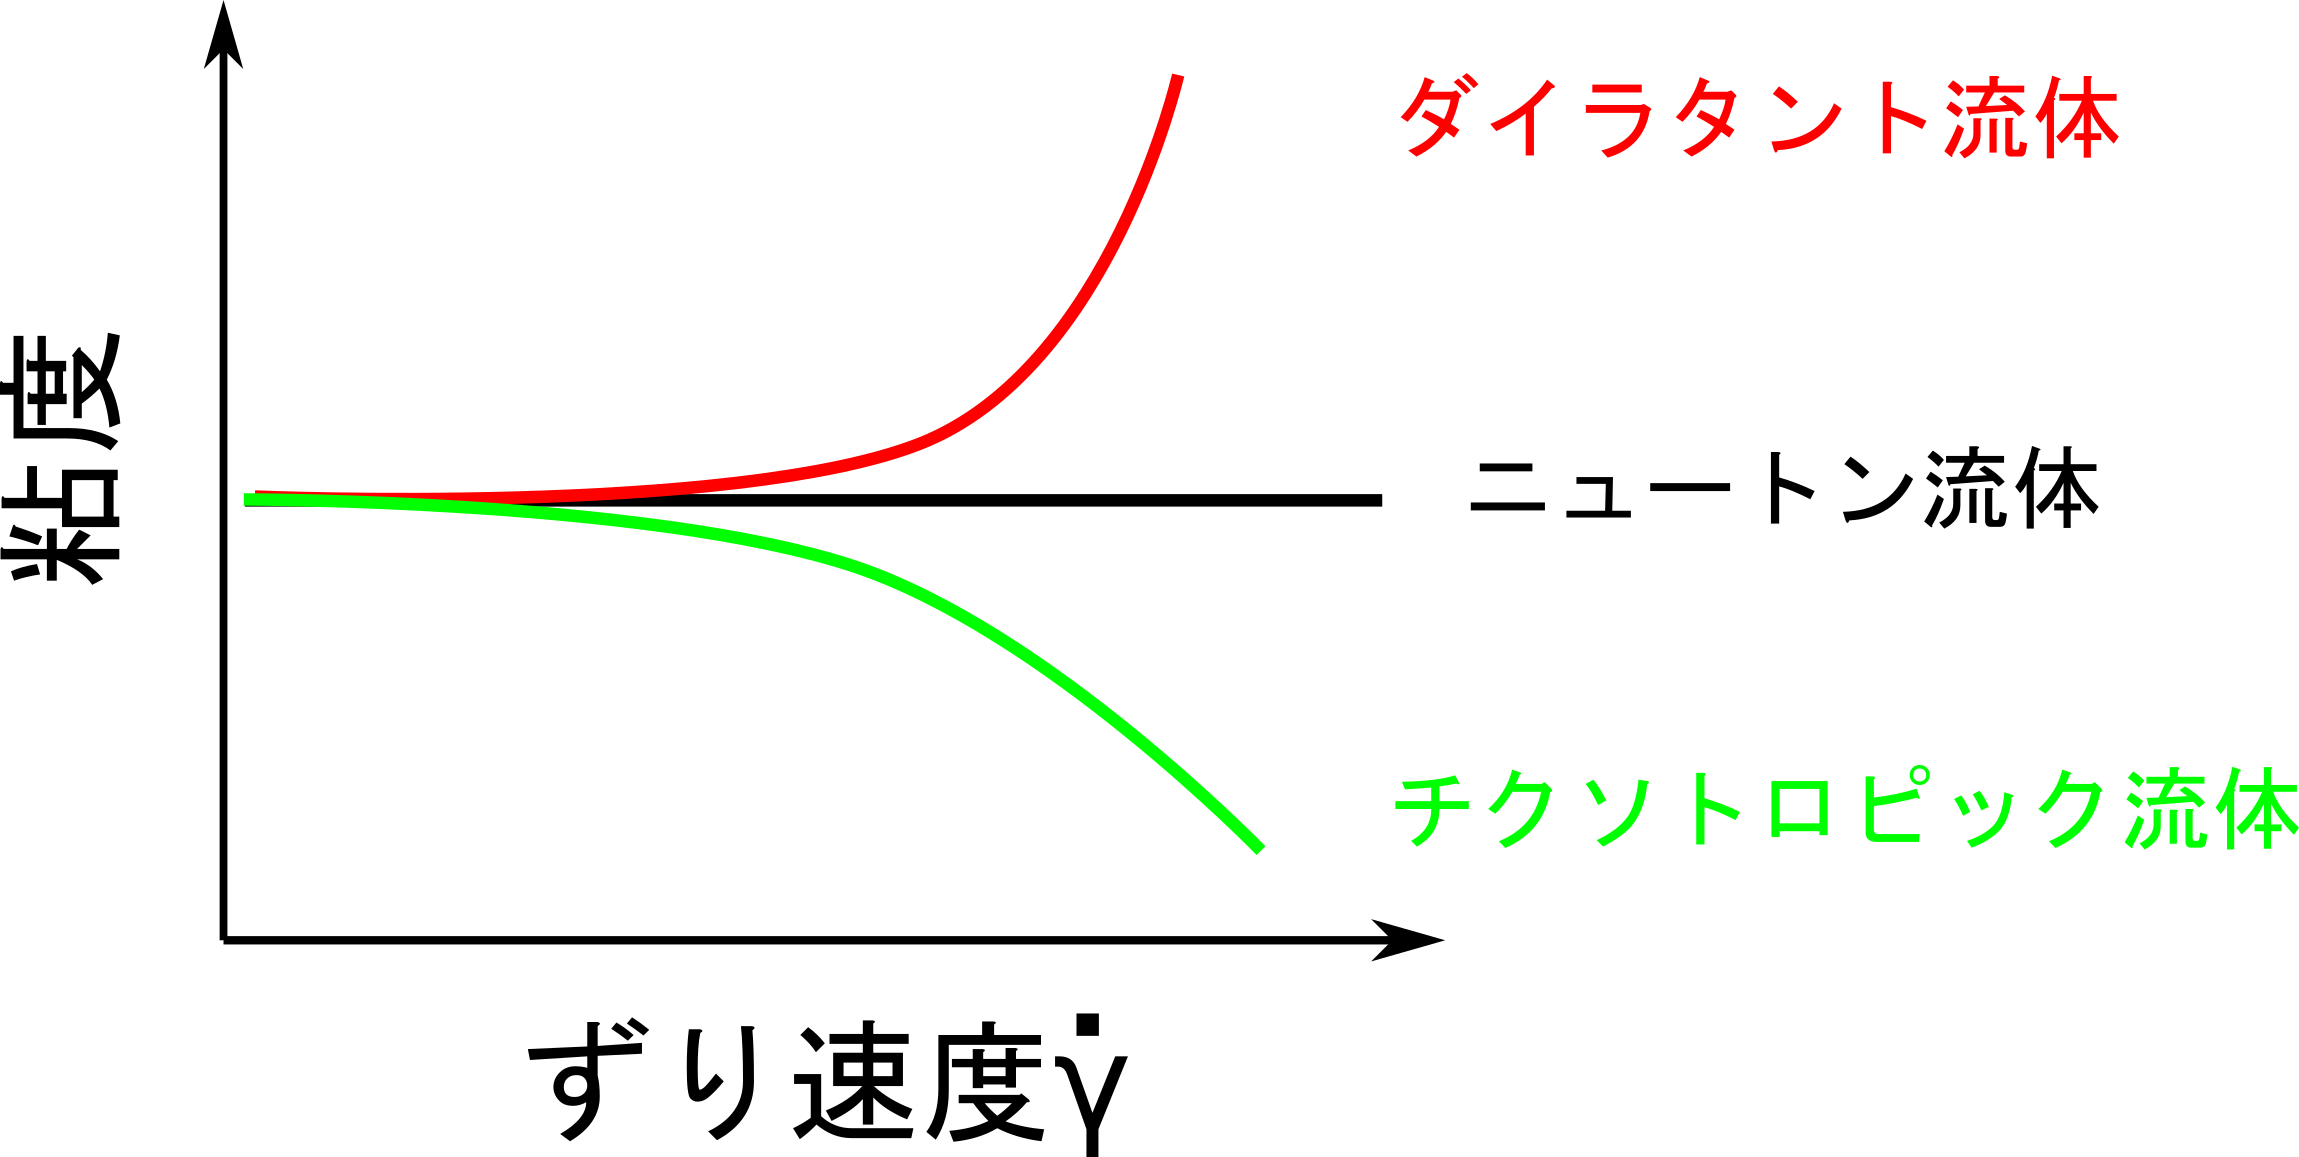
\includegraphics[width=\textwidth]{non_newtonian_3.png}

			\vspace{20pt}

			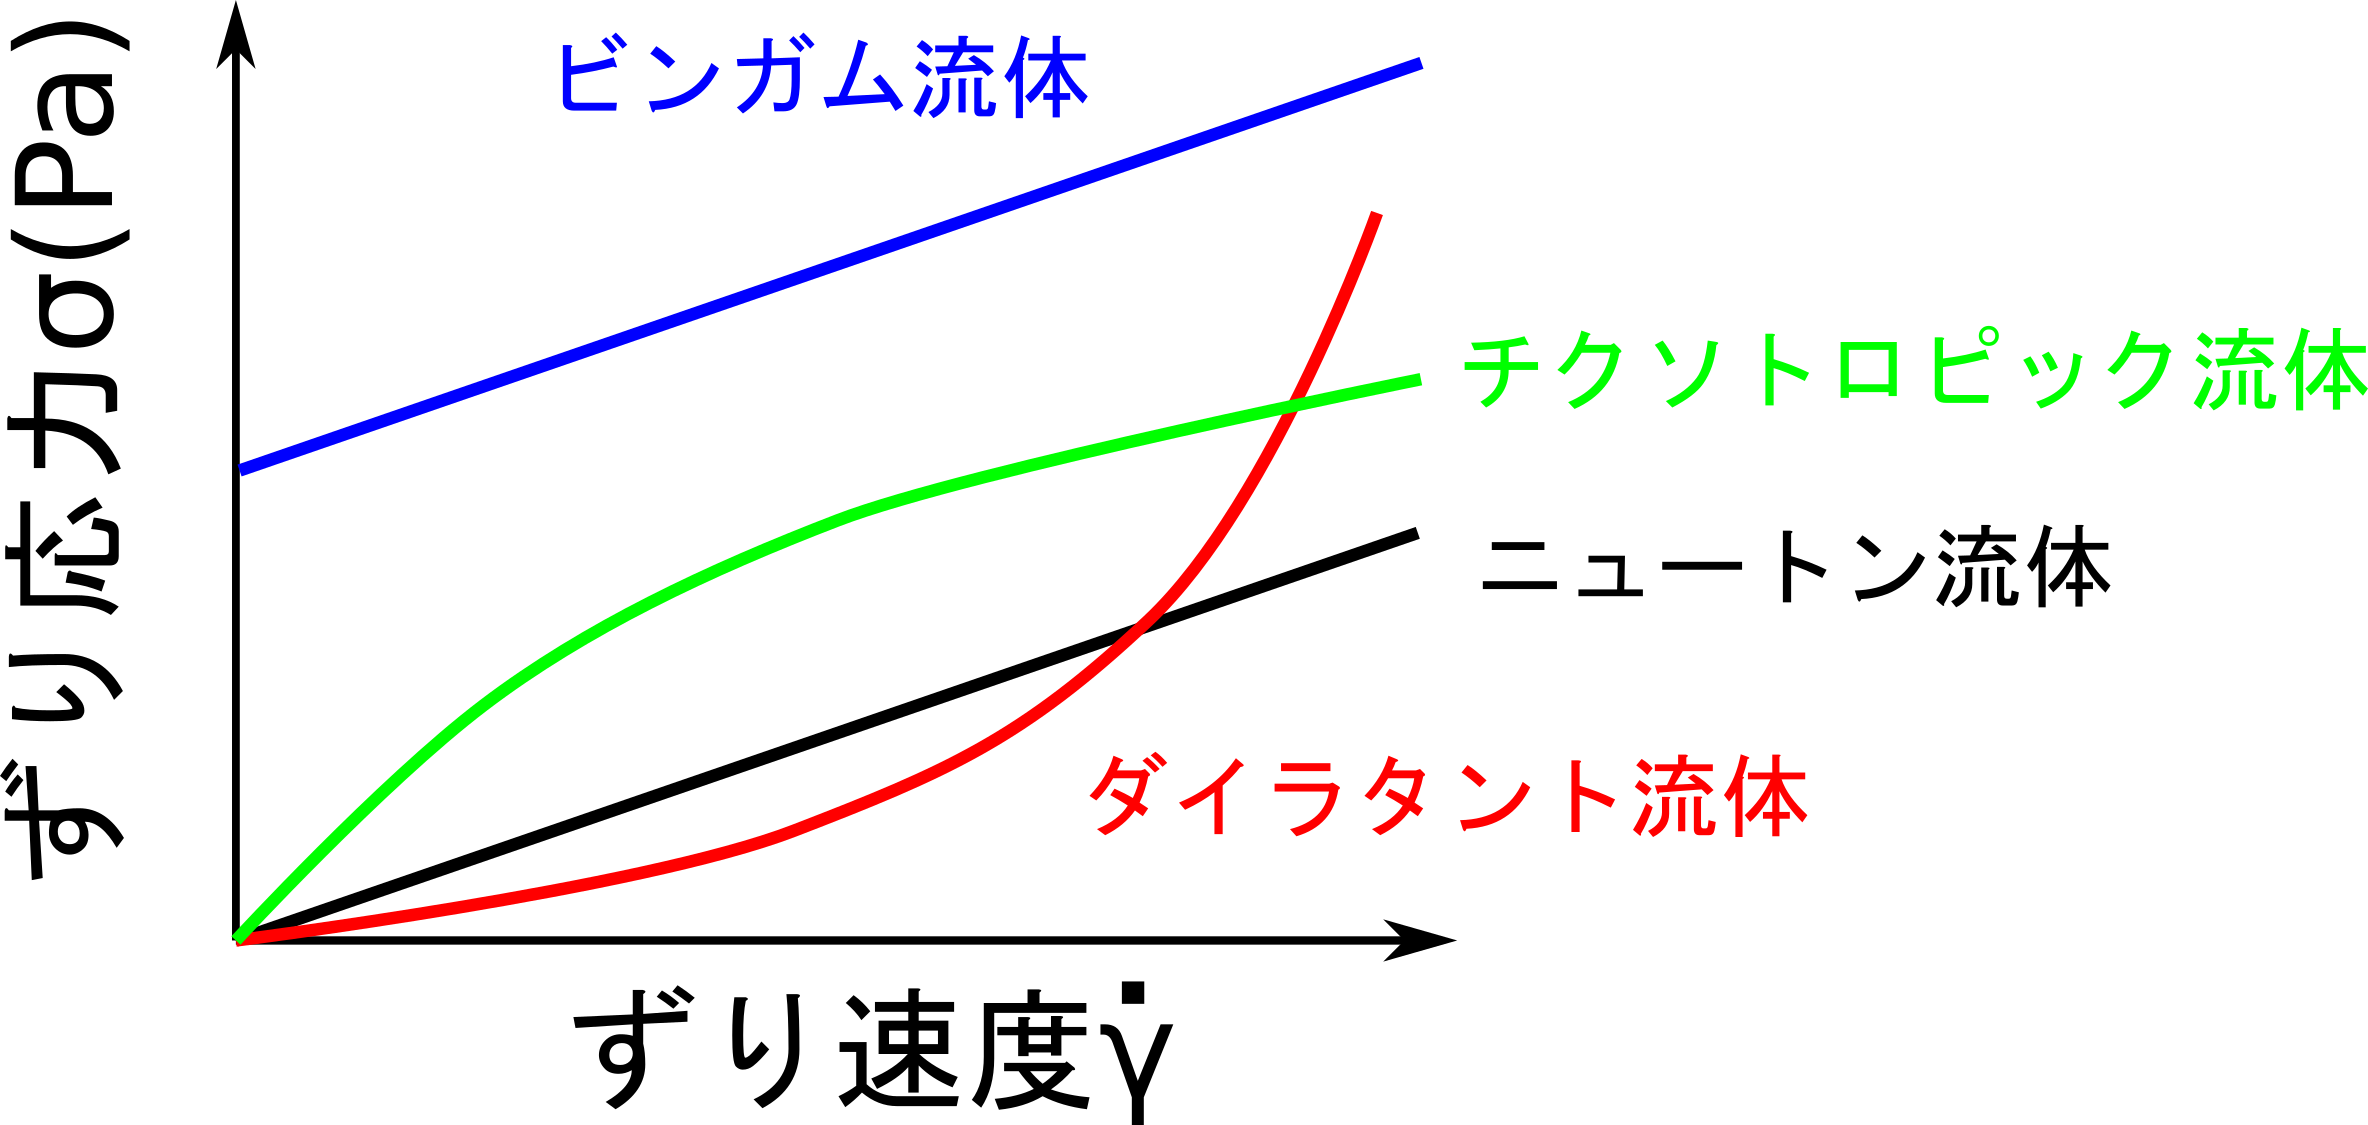
\includegraphics[width=\textwidth]{non_newtonian.png}
			\end{center}
		\end{minipage}
		\begin{minipage}{0.45\textwidth}
			\begin{itemize}
				\item ひずみ速度の変化に対して、以下の2つに大まかに分類
				\begin{itemize}
					\item シア・シニング
					\begin{itemize}
						\item チクソトロピック流体
						\item せん断速度の増加により粘度低下
					\end{itemize}
					\item シア・シックニング
					\begin{itemize}
						\item ダイラタント流体
						\item せん断速度の増加により粘度上昇
					\end{itemize}
				\end{itemize}
				\item (参考)ニュートン流体
					\begin{itemize}
						\item 粘度がせん断速度に依存しない。
						\item せん断速度が上がれば、応力は増加することに注意。
					\end{itemize}
			\end{itemize}
		\end{minipage}
		\caption{せん断速度依存性による分類}
		\label{fig:shearrate_dep}
	\end{center}
\end{figure}

\subsection{シア・シニングについて}

\subsubsection{チクソトロピック流動}
せん断速度の上昇に従って粘度が低下する事象がシア・シニングであり、チクソトロピック流動とも呼ばれています。
\begin{figure}[htb]
	\begin{center}
		\begin{minipage}{0.45\textwidth}
			\begin{itembox}[l]{シア・シニングの挙動}
				\begin{itemize}
					\item 静置状態では内部構造が形成されて高粘度。
					\item 高せん断速度が付与されると、
					\begin{itemize}
						\item 内部構造が崩壊し粘度低下。
					\end{itemize}
					\item せん断速度の低下により、粘度が再上昇。
				\end{itemize}
			\end{itembox}
		\end{minipage}
		\begin{minipage}{0.45\textwidth}
			\begin{center}
			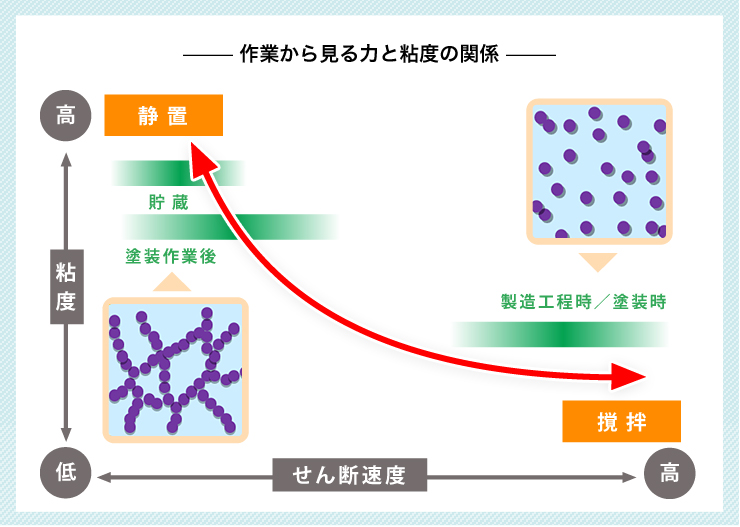
\includegraphics[width=\textwidth]{thixotropy_1w.jpg}
			\end{center}
		\end{minipage}
		\caption{シア・シニングについて}
		\label{fig:shear_thinning}
	\end{center}
\end{figure}
この挙動は、図 \ref{fig:shear_thinning} に示しましたように、外部からのせん断が付与されていない状態において
液体内部では添加粒子が比較的大きな構造を形成することで粘度が高くなっており、
せん断変形が付与されたときには、その内部構造が崩壊することで粘度が低下します。
一旦、内部構造が崩壊しても、再度、静置することで内部構造が再形成されて粘度が上昇します。

\subsubsection{塗膜の液垂れ防止}
このような挙動は、例えば、塗装工程等で重要であり、この特性を上手に設計することで塗膜の液垂れを防止することができるようになります。
具体的には、生地状態に復帰したときの内部構造の再構築に必要な特徴的な時間を短くすることが大事になります。

\begin{figure}[htb]
	\begin{center}
		\begin{minipage}{0.45\textwidth}
			\begin{itembox}[l]{塗膜の液垂れ}
				\begin{itemize}
					\item 塗布後に低せん断速度に復帰したときに、
					\begin{itemize}
						\item 内部構造の再形成が遅くて、
						\item 塗料の粘度が低すぎた場合、
					\end{itemize}
					\item 塗膜の液垂れが生じる。
				\end{itemize}
			\end{itembox}
		\end{minipage}
		\begin{minipage}{0.45\textwidth}
			\begin{center}
			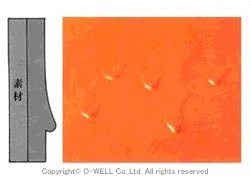
\includegraphics[width=\textwidth]{ekidare.jpg}
			\end{center}
		\end{minipage}
		\caption{塗膜の液垂れ}
		\label{fig:ekidare}
	\end{center}
\end{figure}

\subsubsection{ビンガム流体}

チクソトロピック流動と類似のシア・シニング挙動として、ビンガム流体と呼ばれるものもあります。

これは、ある一定の力がかかるまでは固体として振る舞いますが、一定以上の応力(降伏値)を超えると流動を始めるものであり、
固体と液体との境目のような挙動を示すものとなります。

その挙動の物理的なメカニズムは、チクソトロピック流体とほぼ類似であり、内部構造が一旦崩壊すると、相互作用が一気に小さくなって、
液体として振る舞うことになるわけです。

具体的な実例としては、バターや歯磨き粉を挙げることができます。
\begin{figure}[htb]
	\begin{center}
		\begin{minipage}{0.5\textwidth}
			\begin{itembox}[l]{ビンガム流体}
				\begin{itemize}
					\item 降伏値を有する流体
					\begin{itemize}
						\item ある一定の力がかかるまでは固体。
						\item 降伏値を超えると流動
					\end{itemize}
					\item チクソトロピック流体とほぼ類似の挙動
					\begin{itemize}
						\item 内部構造が一旦崩壊すると、相互作用が一気に小さく。
					\end{itemize}
				\end{itemize}
			\end{itembox}
			
		\end{minipage}
		\begin{minipage}{0.4\textwidth}
			\begin{center}
			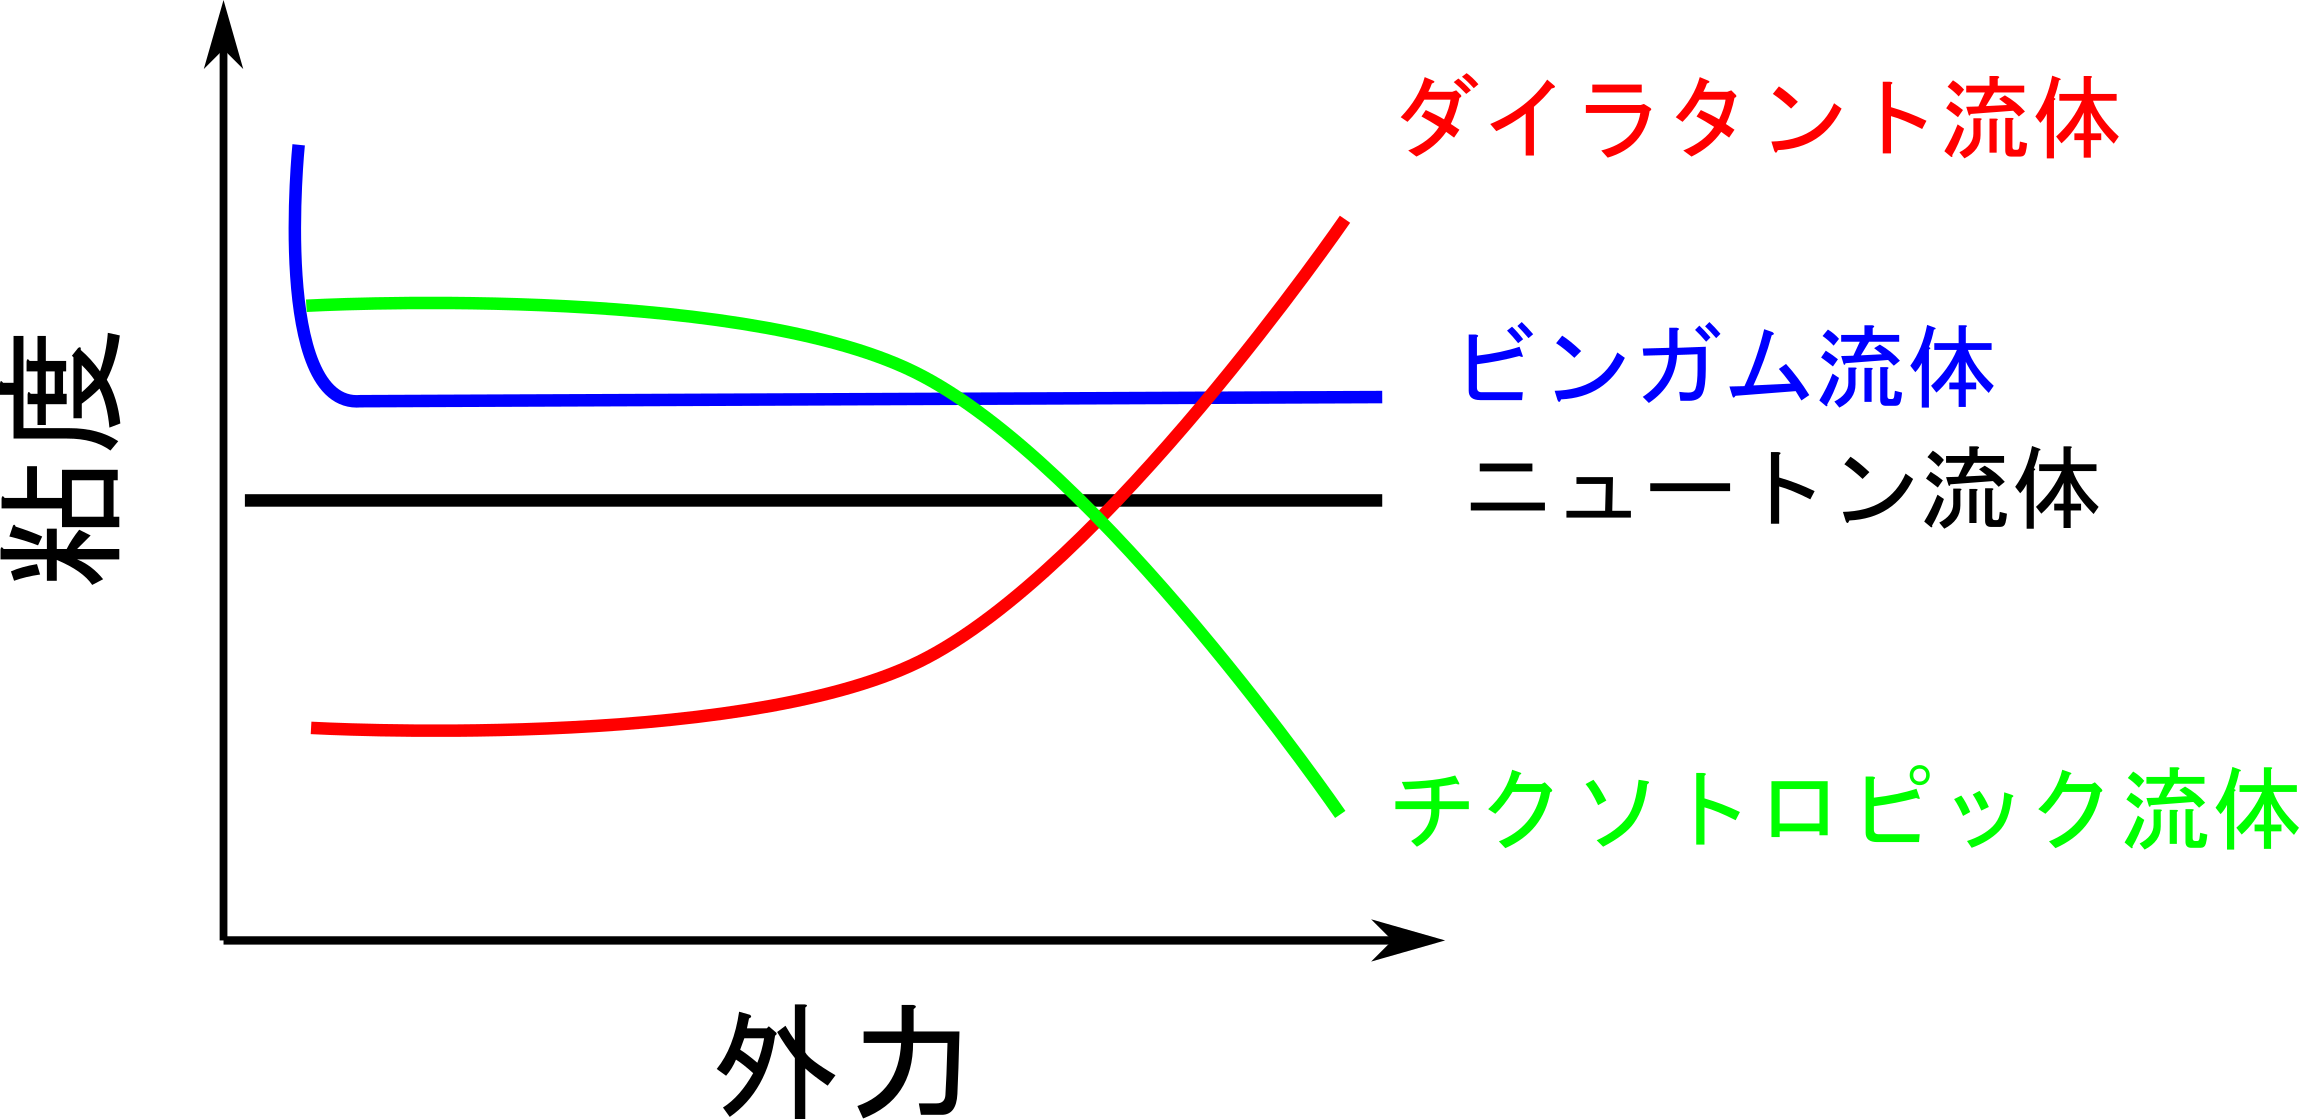
\includegraphics[width=1.2\textwidth]{non_newtonian_2.png}
			\end{center}
		\end{minipage}
		\caption{ビンガム流体について}
		\label{fig:bingham}
	\end{center}
\end{figure}

\subsection{シア・シックニングについて}

シア・シックニング現象として、最もよく知られているものはダイラタンシーと呼ばれるものです。

これは、チクソトロピー流体とは逆の挙動として、遅いせん断変形には液体のように振る舞い、
より速いせん断変形に対してはあたかも固体のような抵抗力を発揮する性質となります。

\begin{figure}[htb]
	\begin{center}
		\begin{minipage}{0.9\textwidth}
			\begin{center}
			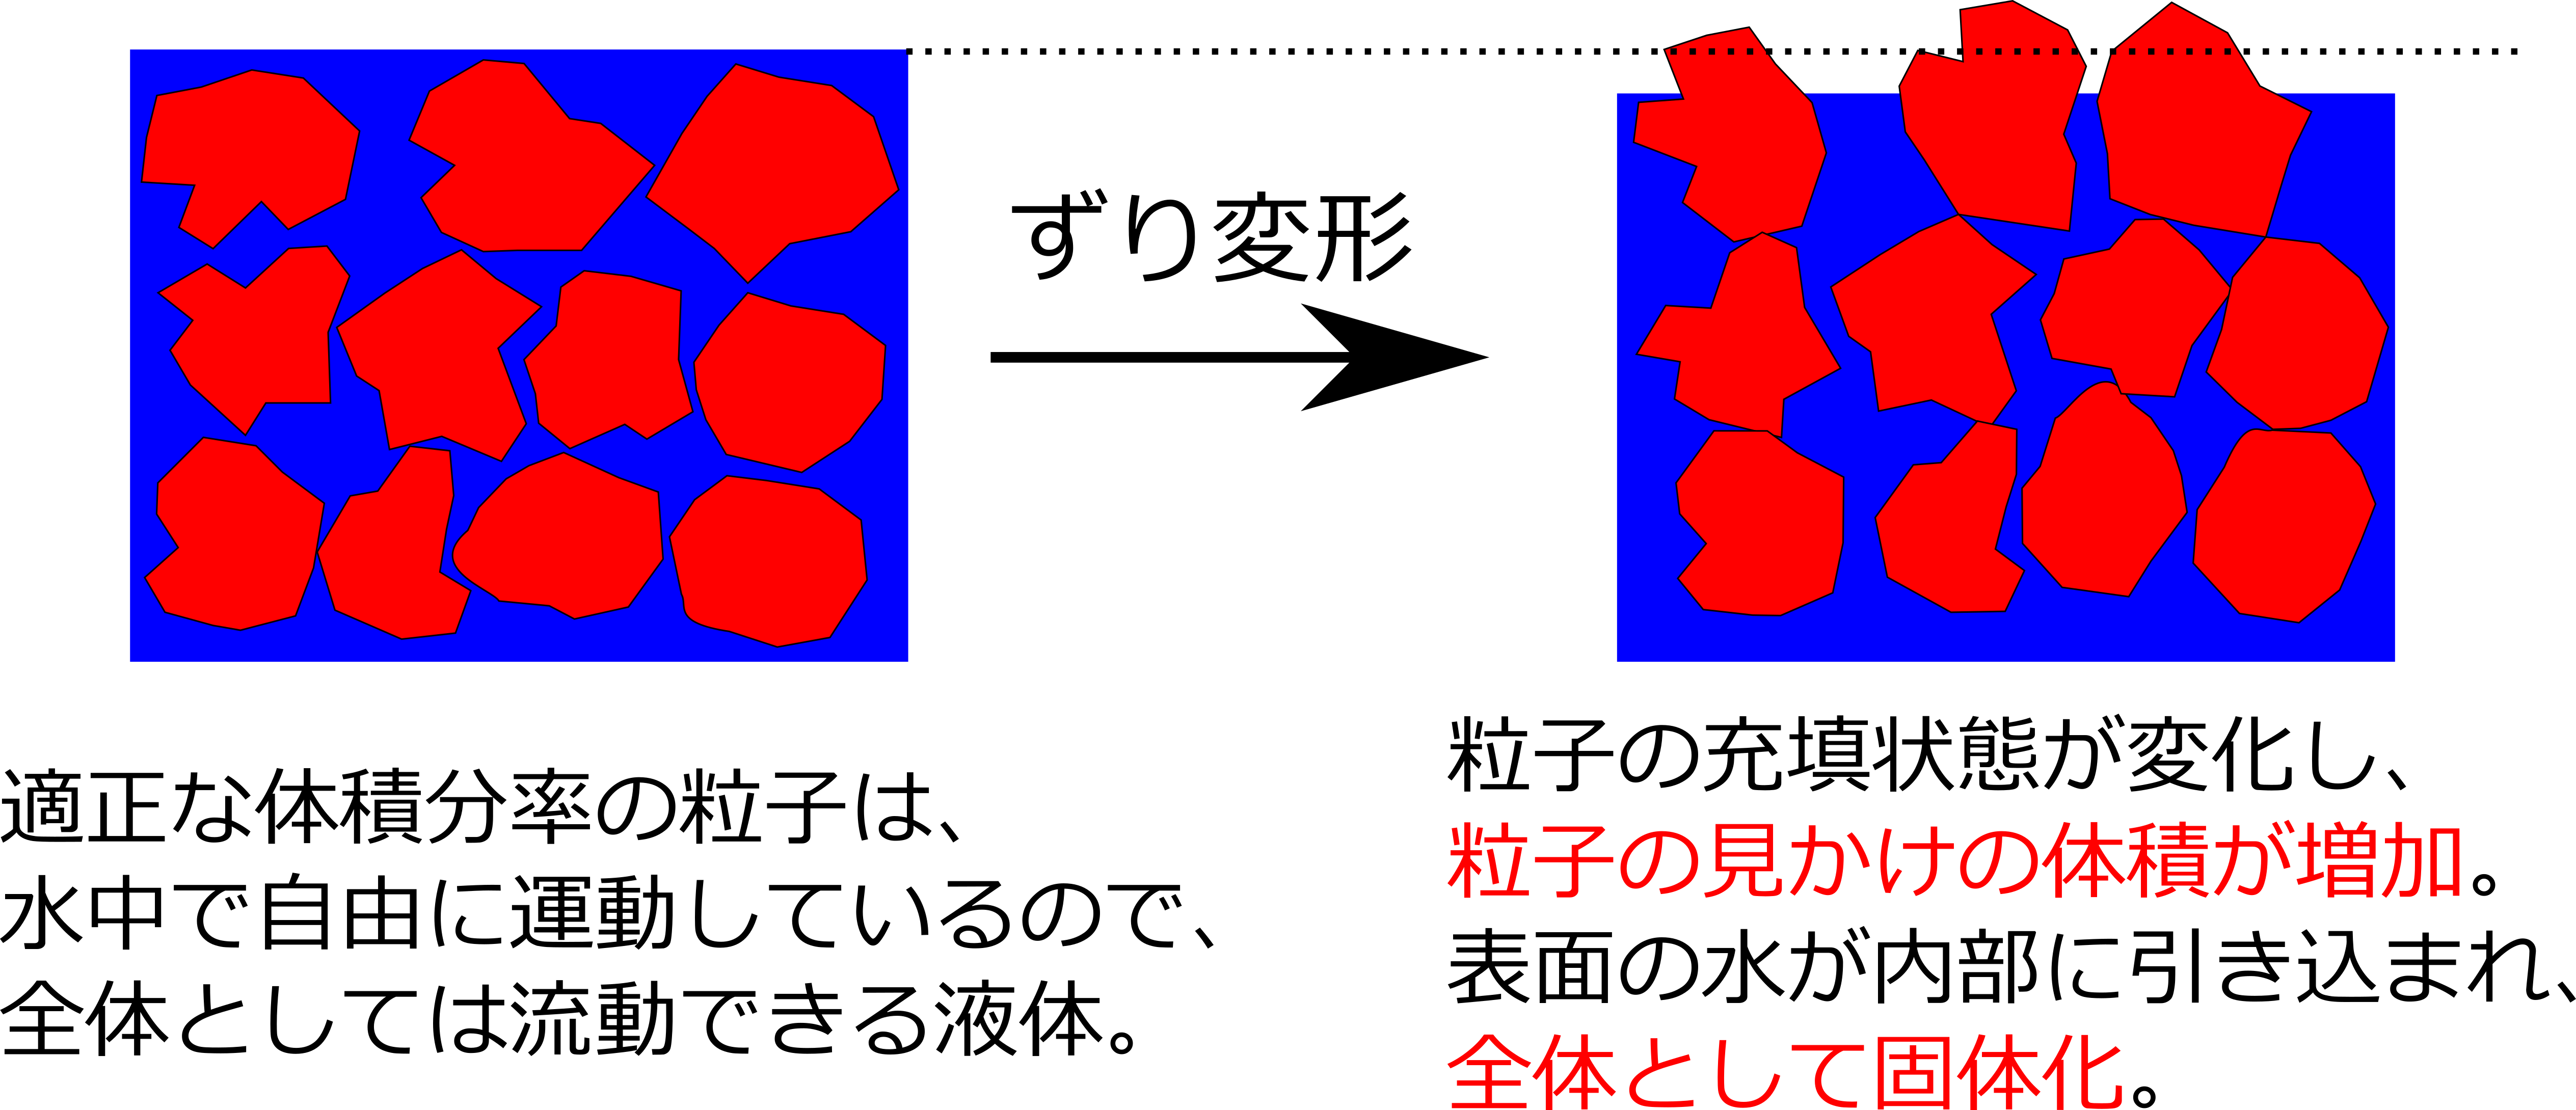
\includegraphics[width=\textwidth]{dilatancy.png}
			\end{center}
		\end{minipage}
		\begin{minipage}{0.9\textwidth}
			\begin{itembox}[l]{ダイラタンシーのメカニズム}
				\begin{itemize}
					\item おなじ大きさの球形粒子の水を吸った状態を考える。
					\item 最密充填では空隙率は26%で、これ以上の水があれば流動。
					\item 急激な外力により単純立方格子になると空隙率は48%になるため、水は全部内部へ吸いこまれる。
					\item こすり合う粒子ができ、体積が幾分膨張し、もろい固体となる。
				\end{itemize}
			\end{itembox}
		\end{minipage}
		\caption{ダイラタンシーについて}
		\label{fig:dilatant}
	\end{center}
\end{figure}

ダイラタンシーは、片栗粉を水に適正量を分散したものをプールに充填して、その上を走り抜けるようなおもしろ実験としてよく知られています。

工業的利用はそれほど報告されていませんが、一つの可能性として、「リキッドアーマー」という名称で検討が行われているようです。
これは、ケブラーに適当なフィラーを充填した分散液を含浸することで、銃弾による急激な衝撃を広い面積で受け止める防弾チョッキ等への応用も
検討されているようですが、未だ実用化には至っていないようです。


\section*{この章のまとめ}

この章では、これまでに行ってきた簡略化したモデルでの議論をベースとして、少しだけ複雑な事象について議論を進めてきました。

実際の事象は非常に複雑なものとなっています。
ここでは、実事象に少しだけ近づくために、流れるということをもう少し詳しく理解することから始めて、
最もシンプルなニュートン流体の流動を表すモデルを振り返りました。

そして、それとの相違という形で、実事象でよく見受けられる複雑な事象を少しだけ理解できるように検討を進めました。
\begin{boxnote}
    \begin{itemize}
		\item 流れるということについて、
		\begin{itemize}
			\item ニュートン流体を見直すために、
			\item 流動を表すモデルをメゾスケールとミクロスケールで見直しました。
		\end{itemize} 
		\item 非ニュートン流体を理解するために、
		\begin{itemize}
			\item ニュートン流体との相違点に着目して、
			\item 非ニュートン性の発現への理解を深めました。
		\end{itemize} 
		\item 最後に、実事象の例を挙げて、以下の振る舞いについての説明を行いました。
		\begin{itemize}
			\item シア・シニングについて
			\item シア・シックニングについて
		\end{itemize}
	\end{itemize}
\end{boxnote}

\clearpage

\question{演習問題 1}
内容を振り返るために、以下に示した文章例の中から適切な記述のものを複数選んでください。
\begin{qlist}
	\qitem 「ニュートン流動」についての、正しい言葉はどれでしょうか?
		\begin{qlist2}
			\qitem せん断応力はせん断速度に比例します。
			\qitem せん断応力はせん断速度には依存しなくて、一定値となります。
			\qitem 粘度は、せん断速度に比例して増加します。
			\qitem ニュートン流体では粘度が一定だから、せん断速度によらずにせん断応力も常に一定となります。
			\qitem ニュートン流体では、せん断速度が変化しても粘度は一定の値となります。
		\end{qlist2}
	\qitem 流動を表す、「水面に板を浮かべたモデル」についての、正しい言葉はどれでしょうか?
		\begin{qlist2}
			\qitem 液体は常に流動するので、板に接している部分でも流れが生じている。
			\qitem 「固体と接している液体は、その相対的な移動速度が同じ」になります。
			\qitem 移動する板と接している液体の層は板と同じ速度で流れます。
			\qitem 水底に接している水も常に流れています。
			\qitem せん断速度と速度勾配は全く異なる単位となっています。
		\end{qlist2}
	\qitem ニュートン流体の「液体のメゾスケールモデル」についての、正しい言葉はどれでしょうか?
		\begin{qlist2}
			\qitem 仮想的な面の間では、応力は発生しません。
			\qitem 仮想的な面の間では、粒子の相互作用に起因するせん断応力が発生しています。
			\qitem ニュートン流体では、仮想的な面の間で生じているせん断応力は、相対的な速度差に比例すると考えることができます。
			\qitem このモデルにおいて、ニュートン流体では粒子間の相互作用はせん断速度に依存しません。
			\qitem このモデルにおいては、ニュートン流体であってもミクロな挙動は粘度とは関係がないことになります。
		\end{qlist2}
	\qitem 非ニュートン流体についての、正しい言葉はどれでしょうか?
		\begin{qlist2}
			\qitem 非ニュートン流体では粘度という考え方を適応することはできません。
			\qitem 実際の液体では、測り方によって粘度の序列は変化する場合があります。
			\qitem 液体とは、どのような測定方法であっても常に流れると考えることができます。
			\qitem 非ニュートン流体では、せん断速度とせん断応力との関係が線形ではありません。
			\qitem 非ニュートン流体では、変形状態(せん断速度や加える力が変化)に依存して粘度が変化します。
		\end{qlist2}
	\qitem 身の回りの実際の液体についての、正しい言葉はどれでしょうか?
		\begin{qlist2}
			\qitem ひずみ速度を増加させた場合に、粘度が増加するような現象をシア・シニングと呼びます。
			\qitem チクソトロピック流体と分類されるものは、ひずみ速度を増加させると粘度が低下します。
			\qitem シア・シックニングとは、ひずみ速度を増加させたときに粘度が上昇する現象のことを指します。
			\qitem シア・シックニングとは、高いひずみ速度において内部構造が崩壊して粘度が低下すると考えられます。
			\qitem 塗料の液垂れ防止には、シア・シニング現象を上手に利用することが必要となります。
		\end{qlist2}
\end{qlist}

\question{演習問題 2}
内容を振り返るために、テキストで用いた言葉を使って簡単な穴埋めを行ってください。
\begin{qlist}
	\qitem 「流動を表すモデル」について、\qbox{(a)}から\qbox{(i)}までのカッコを埋めてください。
		\vspace{5mm}
		\begin{qlist2}
			\qitem 「流動を表すモデル」について
			\begin{center}
				\begin{minipage}{0.4\textwidth}
					\begin{itembox}[l]{水面に板を浮かべたモデル}
						\begin{itemize}
							\item 水深方向に n+1 層に分割
								\begin{itemize}
									\item 水面の板との境目を0
									\item 水底との境目を n 
								\end{itemize}
								\item 液体の内部では、
								\begin{itemize}
									\item 水深に応じて流れる速度の分布
									\item 最も単純な状態:\\速度勾配が一定
								\end{itemize}
						\end{itemize}
					\end{itembox}
				\end{minipage}
				\begin{minipage}{0.45\textwidth}
					\begin{center}
					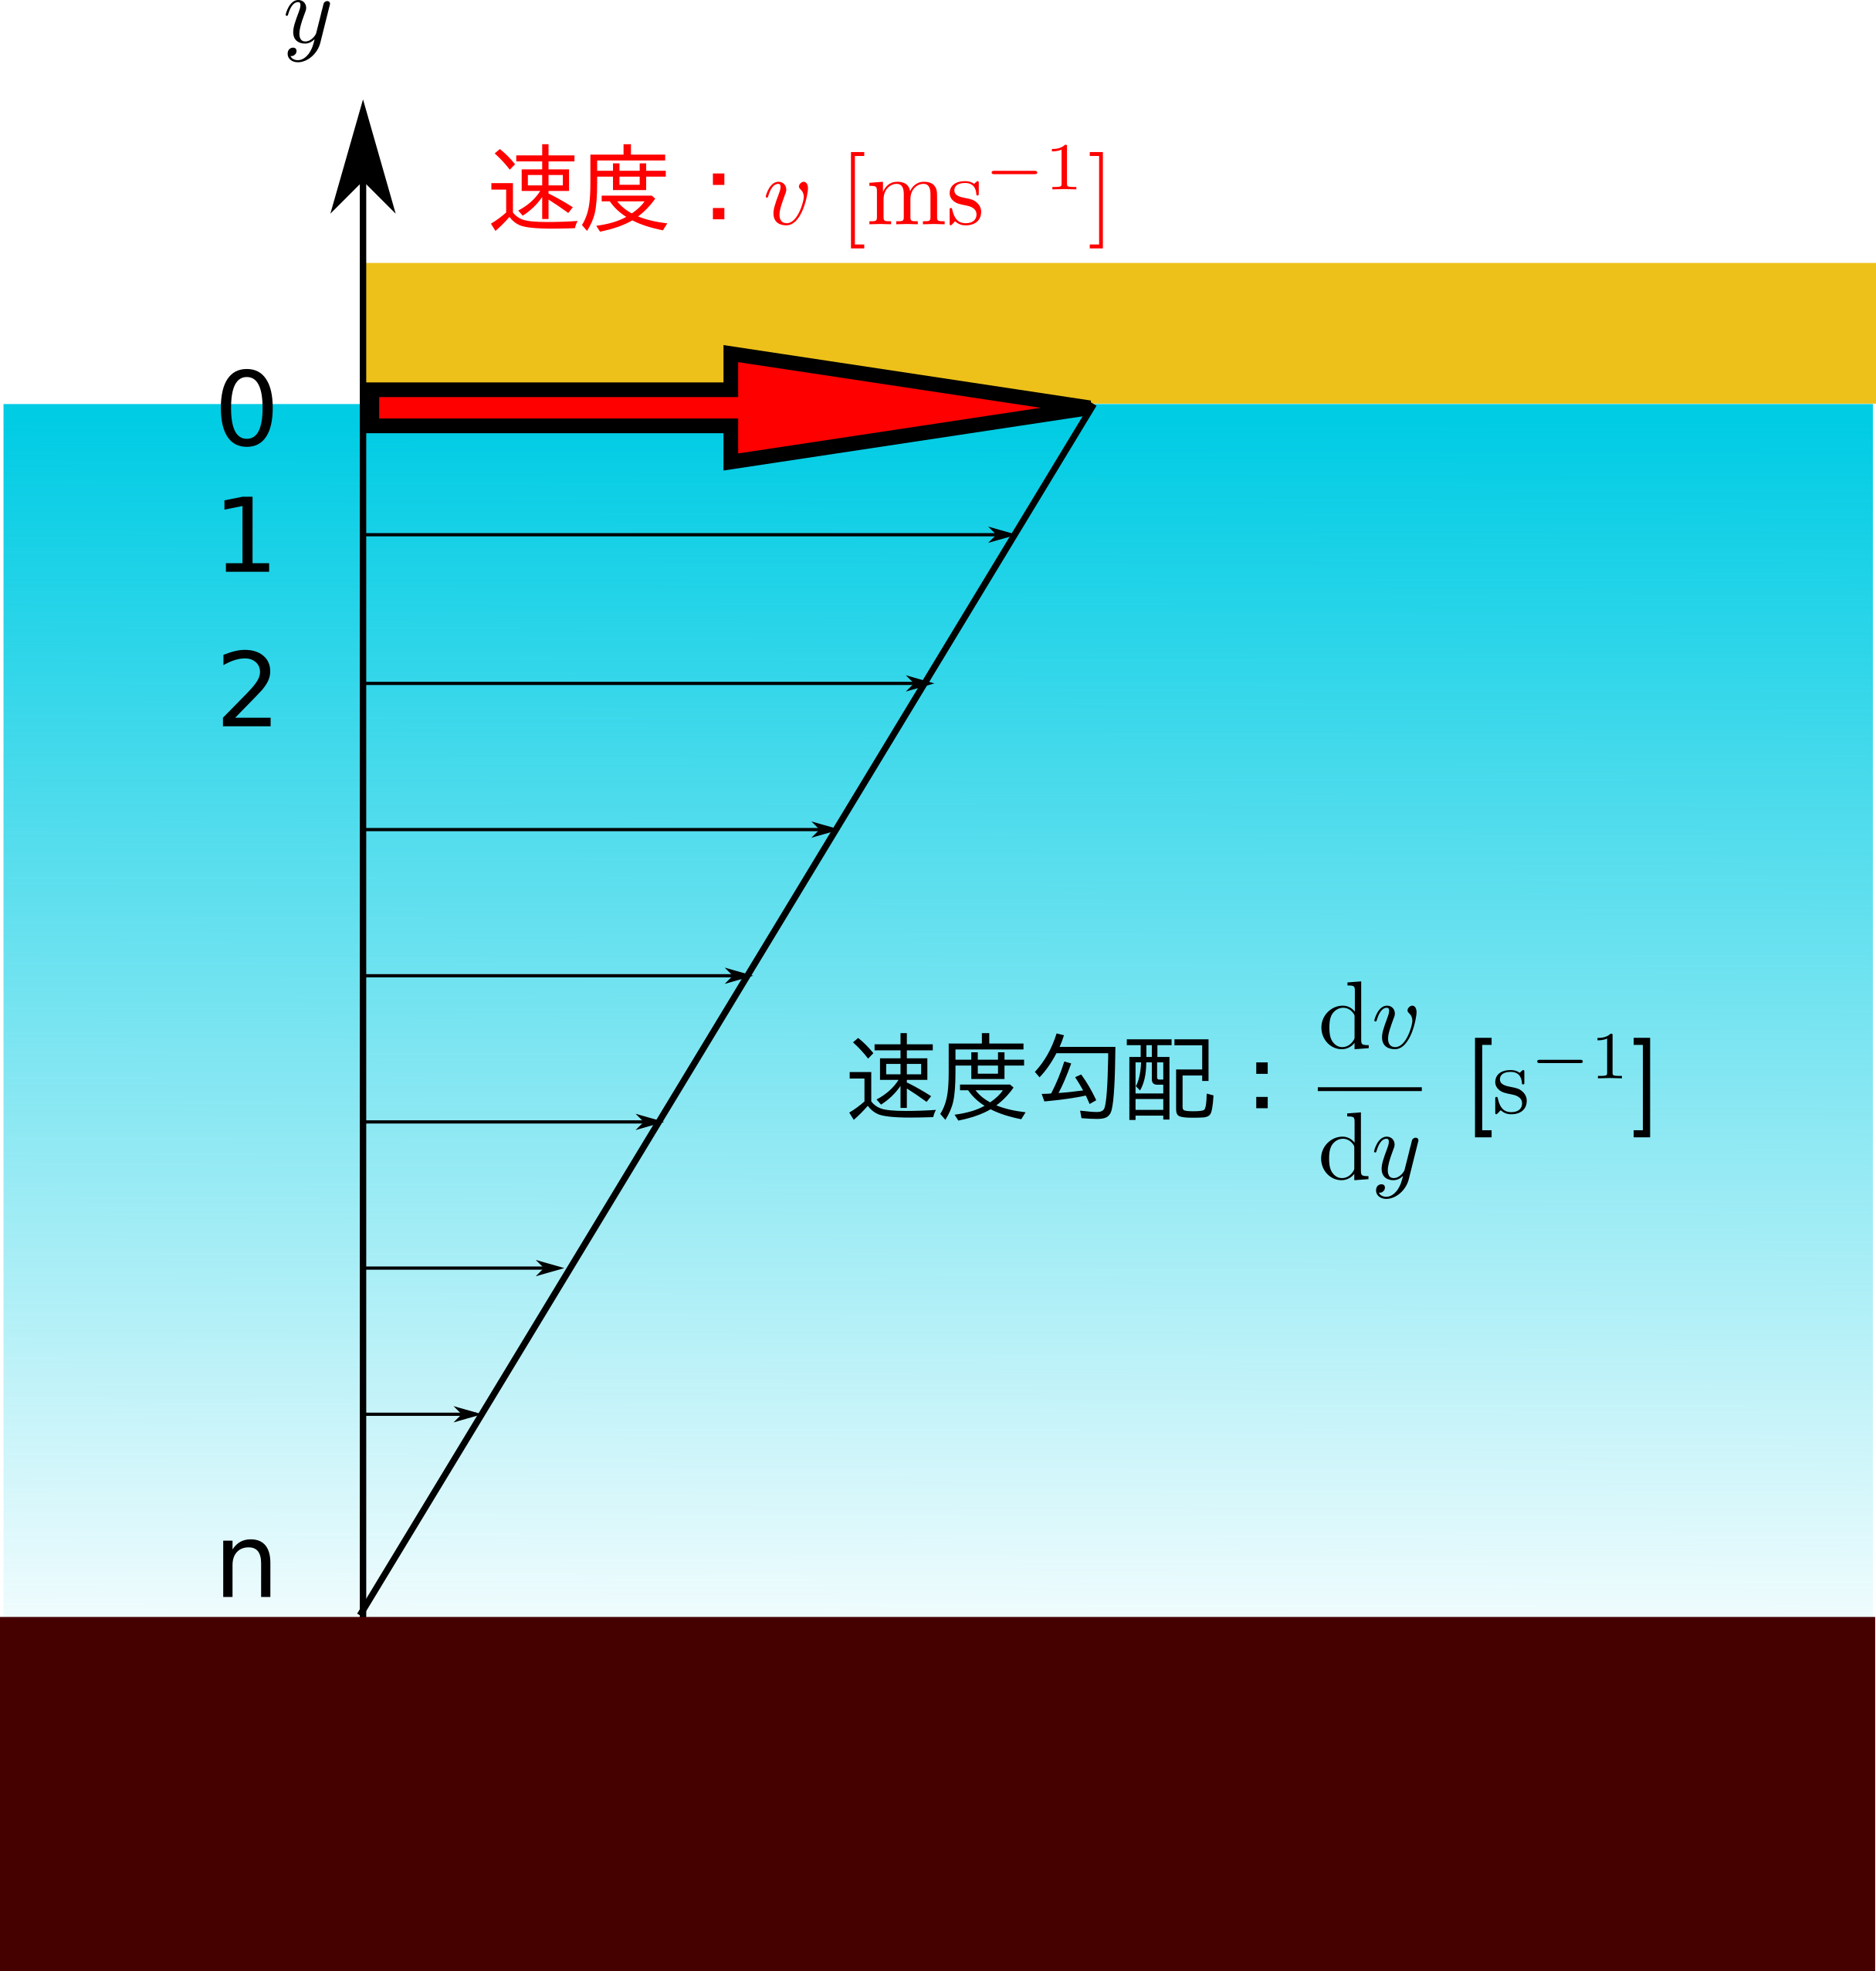
\includegraphics[width=.75\textwidth]{shear_3.png}
					\end{center}
				\end{minipage}
				\begin{minipage}{0.9\textwidth}
					\begin{center}
					\begin{itembox}[l]{注意すべきポイント}
						\begin{itemize}
							\item 固体と接している液体は、その相対的な\qbox{}が同じ。
							\begin{itemize}
								\item 移動する板と接している層 0 は板と同じ速度 $v$ で流れ、
								\item 地面に接している層 $n$ は\qbox{}。
							\end{itemize}
							\item 評価の対象である液体の内部では、
							\begin{itemize}
								\item 水深に応じて、流れる速度の\qbox{}が生じる。
							\end{itemize}
							\item 液体の流れる速度は、
							\begin{itemize}
								\item 水深 $y$ の関数として $v(y)$
								\item \qbox{}と呼ばれ、その単位は $[\mathrm{s^{-1}}]$
							\end{itemize}
						\end{itemize}
					\end{itembox}
					\end{center}
				\end{minipage}
			\end{center}
			
			\vspace{5mm}
			\qitem ニュートン流体について
			\begin{center}
				\begin{minipage}{0.9\textwidth}
					\begin{center}
					\begin{itembox}[l]{ニュートン流体の特徴}
						\begin{itemize}
							\item 「流動を表すモデル」において、速度勾配が\qbox{}となっている。
							\item 速度勾配に従って、各層ごとに\qbox{}が発生
							\begin{itemize}
								\item その値は、局所的なせん断速度に比例して\qbox{}。
								\item 逆に言えば、\qbox{}によらずに\qbox{}が一定。
							\end{itemize}
						\end{itemize}
					\end{itembox}
					\end{center}
				\end{minipage}
			\end{center}

		\end{qlist2}

		\begin{itembox}[l]{選択肢}
			\begin{center}
				\begin{tabular}{lllll}
					1. 分布	&2. せん断応力 &3. 流れない	&4. 速度勾配	&5. 粘度\\
					6. 一定	&7. 変化  &8. せん断速度	&9. 移動速度
				\end{tabular}
			\end{center}
		\end{itembox}
\end{qlist}

\begin{qlist}
	\qitem 「非ニュートン流体」について、\qbox{(j)}から\qbox{(s)}までのカッコを埋めてください。

			\vspace{3mm}
			\begin{qlist2}
			\qitem 非ニュートン流体とは
			\begin{center}
				\begin{minipage}{0.9\textwidth}
					\begin{itembox}[l]{非ニュートン流体とは?}
						\begin{itemize}
							\item 簡単に言えば、ニュートン流動と異なる流動特性を示すものを指します。
							\begin{itemize}
								\item せん断応力が\qbox{}ではない。
								\item 変形状態(せん断速度や加える力が変化)に依存して、\qbox{}が変化する。
							\end{itemize}
							\item その原因は多数あるが、基本的に内部に\qbox{}を有する物質で生じる。
						\end{itemize}
					\end{itembox}
				\end{minipage}

				\vspace{4mm}

				\begin{minipage}{0.43\textwidth}
					\begin{center}
					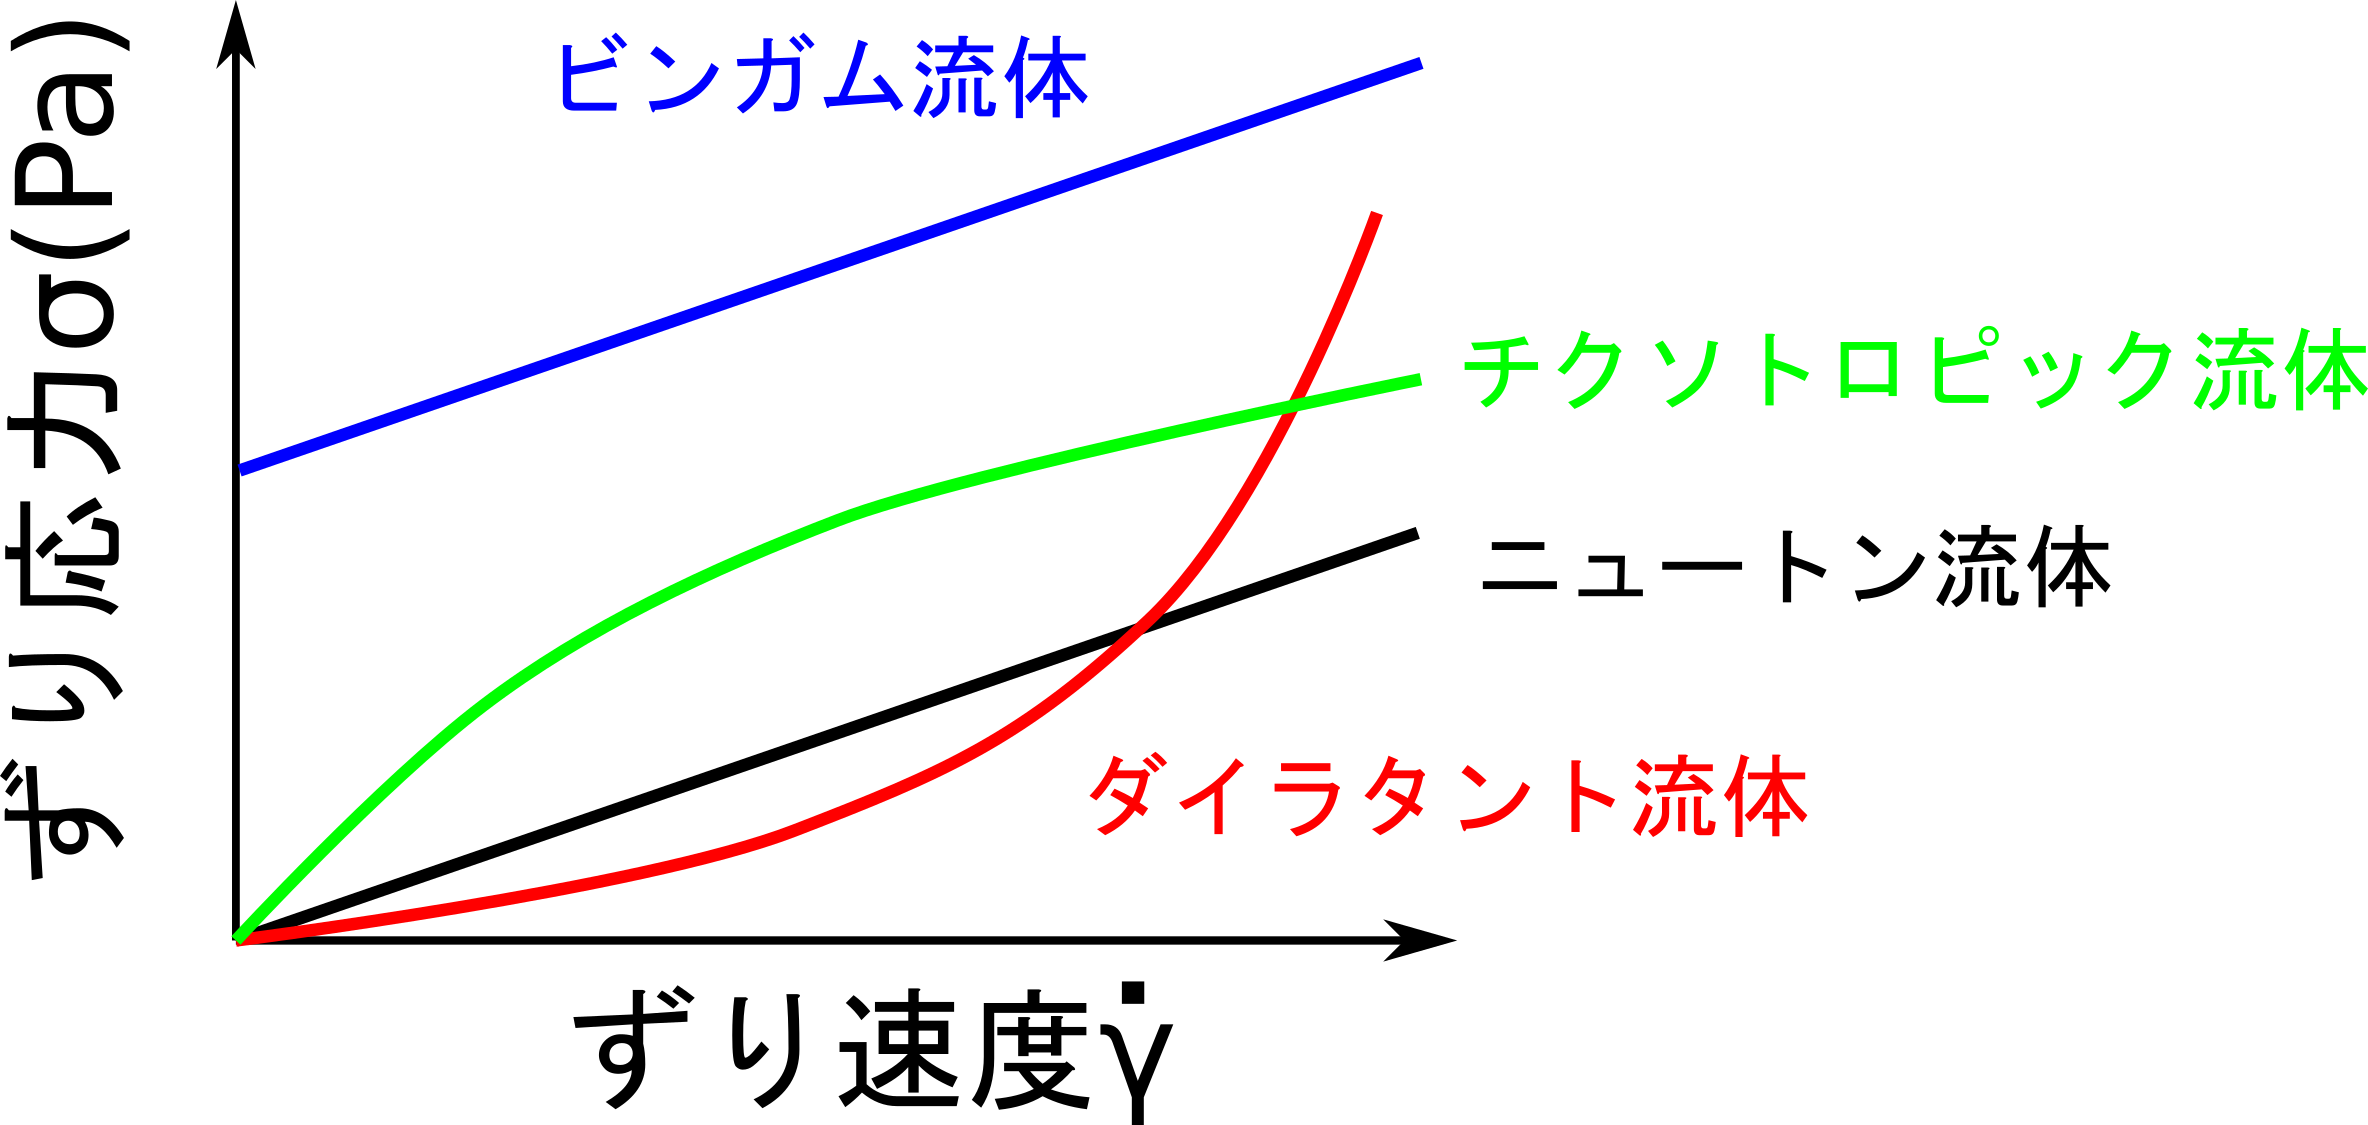
\includegraphics[width=\textwidth]{non_newtonian.png}
					\end{center}
				\end{minipage}
				\begin{minipage}{0.43\textwidth}
					\begin{center}
					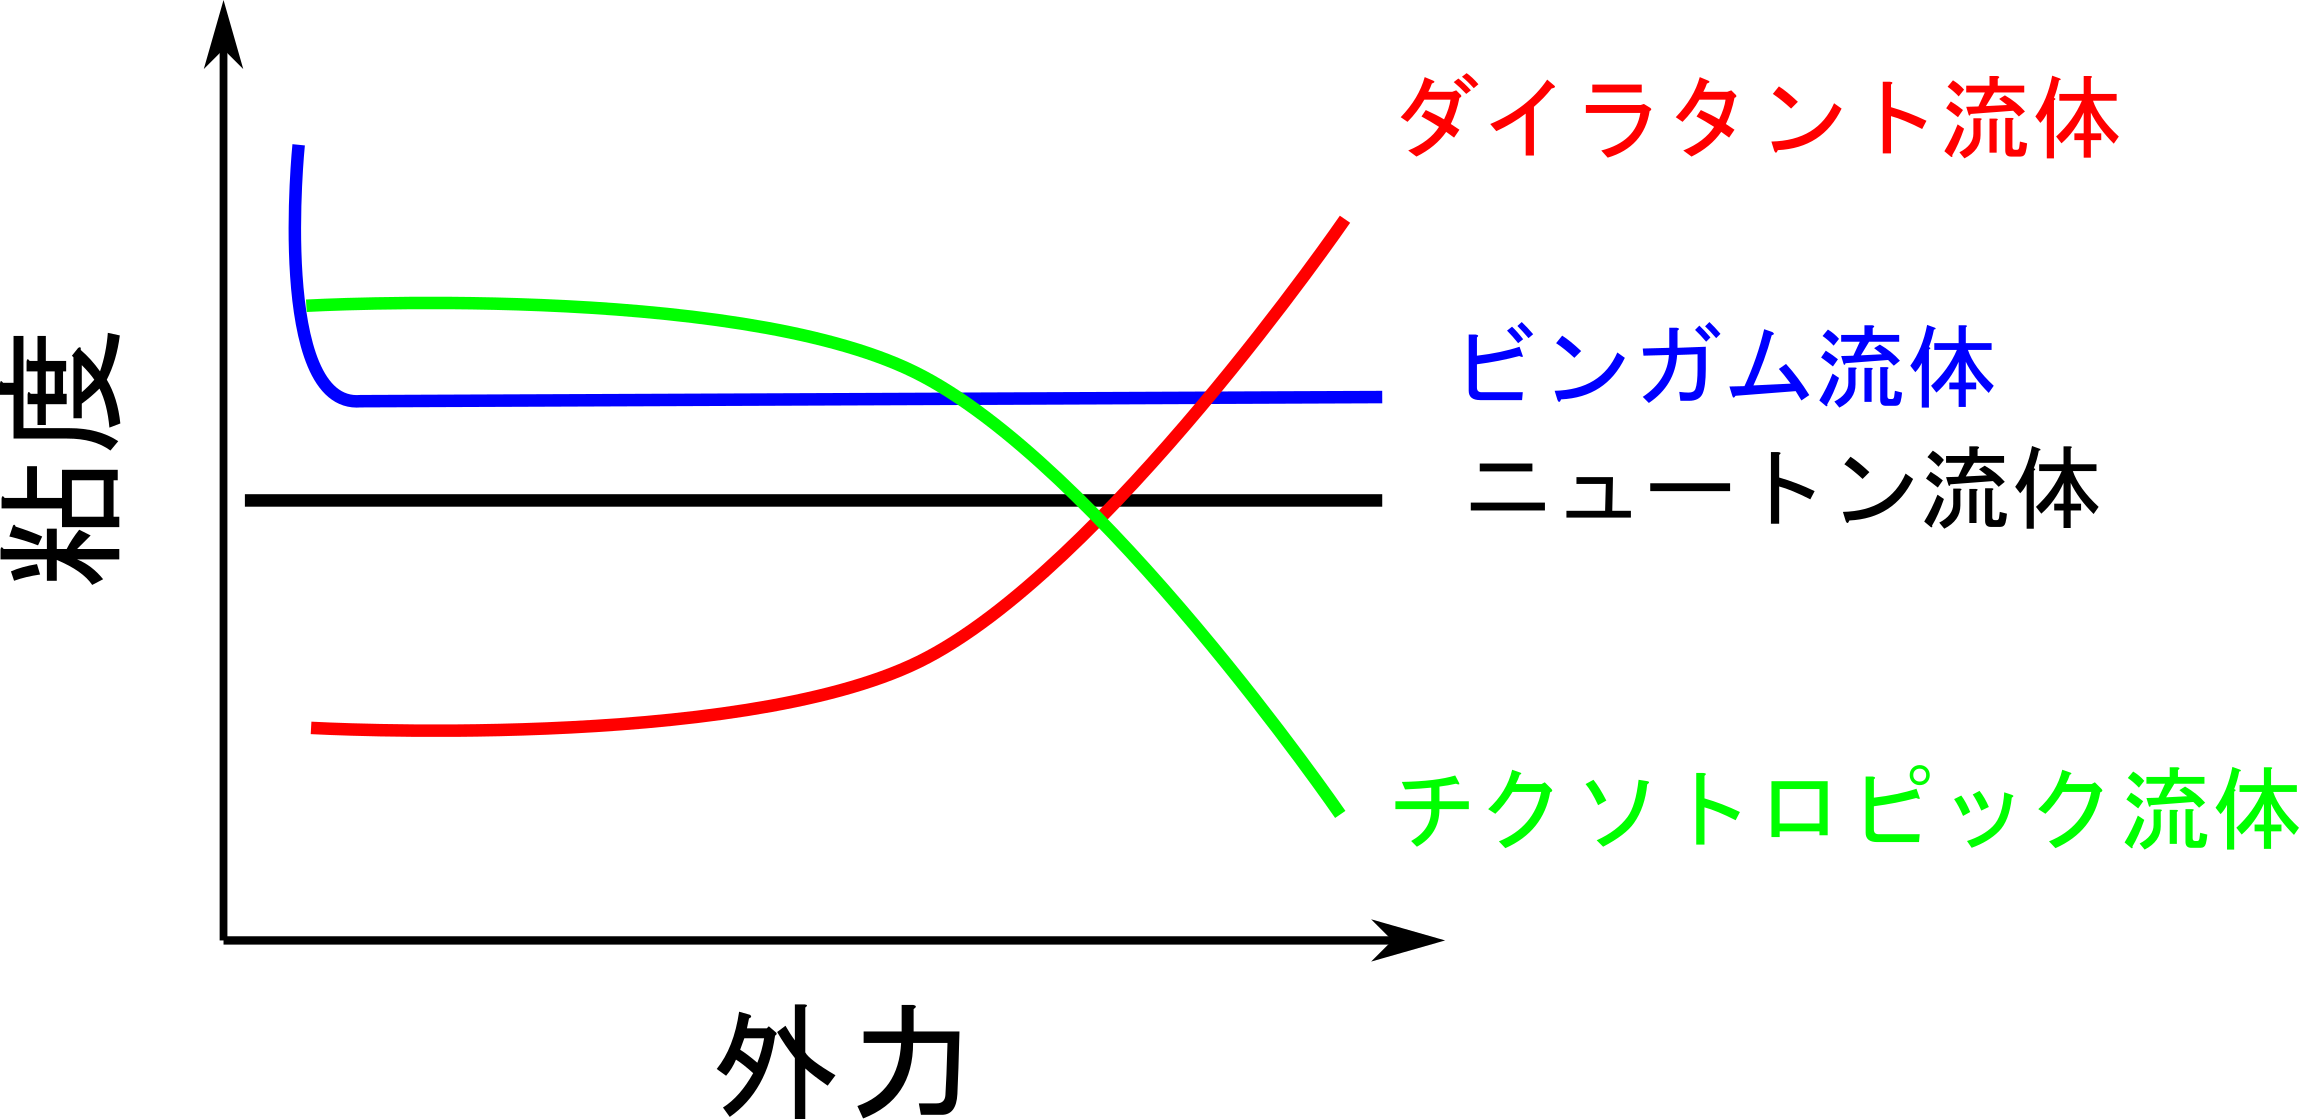
\includegraphics[width=\textwidth]{non_newtonian_2.png}
					\end{center}
				\end{minipage}
			\end{center}

			\vspace{3mm}
			\qitem 非ニュートン流体の発現理由
			\begin{itemize}
				\item 系の挙動を支配する特徴的な時間とは?
				\begin{itemize}
					\item 物質の\qbox{}に由来する特徴的時間が存在し、
					\item これは、内部構造が\qbox{}、再構築するための特徴的な時間と考える。
				\end{itemize}
				\item 外部からの\qbox{}に関わる時間(変形に関与する時間)との関係
				\begin{itemize}
					\item 物質中の内部構造が持つ特徴的な時間よりも短い時間(速い速度)で変形すると、
					\item 内部構造が\qbox{}するため巨視的な粘度が変化し、非ニュートン性が発現する。
				\end{itemize}
			\end{itemize}
			
			\vspace{3mm}
			\qitem シア・シニング(チクソトロピー流体)について
			\begin{center}
				\begin{minipage}{0.5\textwidth}
					\begin{itembox}[l]{シア・シニングの挙動}
						\begin{itemize}
							\item \qbox{}では内部構造が形成されて高粘度。
							\item 高せん断速度が付与されると、
							\begin{itemize}
								\item 内部構造が崩壊し粘度が\qbox{}
							\end{itemize}
							\item せん断速度の低下により粘度が、\qbox{}。
						\end{itemize}
					\end{itembox}
				\end{minipage}
				\begin{minipage}{0.38\textwidth}
					\begin{center}
					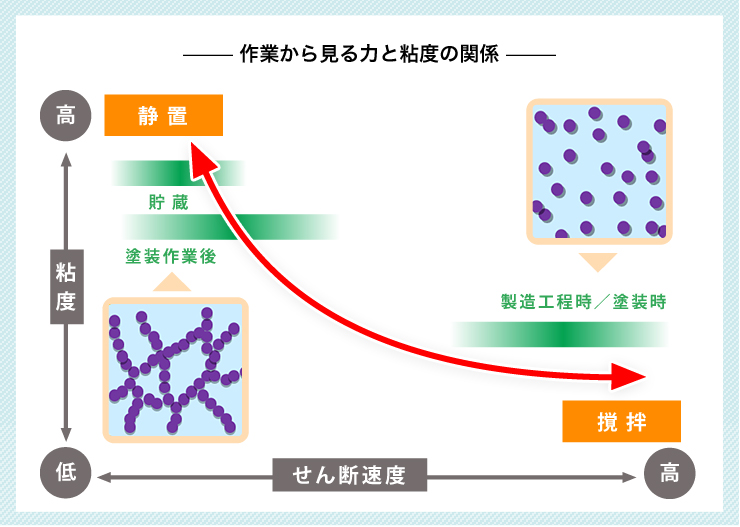
\includegraphics[width=1.2\textwidth]{thixotropy_1w.jpg}
					\end{center}
				\end{minipage}
			\end{center}

		\end{qlist2}

		\begin{itembox}[l]{選択肢}
			\begin{center}
				\begin{tabular}{lllll}
					1. 内部構造	&2. 粘度	&3. 構造	&4. 低下 &5. 再上昇\\
					6. 静置状態	&7. 崩壊	&8. 変形	&9. 線形 &10. 変化
				\end{tabular}
			\end{center}
		\end{itembox}
\end{qlist}


\end{document}